% Options for packages loaded elsewhere
% Options for packages loaded elsewhere
\PassOptionsToPackage{unicode}{hyperref}
\PassOptionsToPackage{hyphens}{url}
\PassOptionsToPackage{dvipsnames,svgnames,x11names}{xcolor}
%
\documentclass[
]{article}
\usepackage{xcolor}
\usepackage{amsmath,amssymb}
\setcounter{secnumdepth}{-\maxdimen} % remove section numbering
\usepackage{iftex}
\ifPDFTeX
  \usepackage[T1]{fontenc}
  \usepackage[utf8]{inputenc}
  \usepackage{textcomp} % provide euro and other symbols
\else % if luatex or xetex
  \usepackage{unicode-math} % this also loads fontspec
  \defaultfontfeatures{Scale=MatchLowercase}
  \defaultfontfeatures[\rmfamily]{Ligatures=TeX,Scale=1}
\fi
\usepackage{lmodern}
\ifPDFTeX\else
  % xetex/luatex font selection
  \setmainfont[]{Noto Sans CJK JP}
\fi
% Use upquote if available, for straight quotes in verbatim environments
\IfFileExists{upquote.sty}{\usepackage{upquote}}{}
\IfFileExists{microtype.sty}{% use microtype if available
  \usepackage[]{microtype}
  \UseMicrotypeSet[protrusion]{basicmath} % disable protrusion for tt fonts
}{}
\makeatletter
\@ifundefined{KOMAClassName}{% if non-KOMA class
  \IfFileExists{parskip.sty}{%
    \usepackage{parskip}
  }{% else
    \setlength{\parindent}{0pt}
    \setlength{\parskip}{6pt plus 2pt minus 1pt}}
}{% if KOMA class
  \KOMAoptions{parskip=half}}
\makeatother
% Make \paragraph and \subparagraph free-standing
\makeatletter
\ifx\paragraph\undefined\else
  \let\oldparagraph\paragraph
  \renewcommand{\paragraph}{
    \@ifstar
      \xxxParagraphStar
      \xxxParagraphNoStar
  }
  \newcommand{\xxxParagraphStar}[1]{\oldparagraph*{#1}\mbox{}}
  \newcommand{\xxxParagraphNoStar}[1]{\oldparagraph{#1}\mbox{}}
\fi
\ifx\subparagraph\undefined\else
  \let\oldsubparagraph\subparagraph
  \renewcommand{\subparagraph}{
    \@ifstar
      \xxxSubParagraphStar
      \xxxSubParagraphNoStar
  }
  \newcommand{\xxxSubParagraphStar}[1]{\oldsubparagraph*{#1}\mbox{}}
  \newcommand{\xxxSubParagraphNoStar}[1]{\oldsubparagraph{#1}\mbox{}}
\fi
\makeatother

\usepackage{color}
\usepackage{fancyvrb}
\newcommand{\VerbBar}{|}
\newcommand{\VERB}{\Verb[commandchars=\\\{\}]}
\DefineVerbatimEnvironment{Highlighting}{Verbatim}{commandchars=\\\{\}}
% Add ',fontsize=\small' for more characters per line
\usepackage{framed}
\definecolor{shadecolor}{RGB}{241,243,245}
\newenvironment{Shaded}{\begin{snugshade}}{\end{snugshade}}
\newcommand{\AlertTok}[1]{\textcolor[rgb]{0.68,0.00,0.00}{#1}}
\newcommand{\AnnotationTok}[1]{\textcolor[rgb]{0.37,0.37,0.37}{#1}}
\newcommand{\AttributeTok}[1]{\textcolor[rgb]{0.40,0.45,0.13}{#1}}
\newcommand{\BaseNTok}[1]{\textcolor[rgb]{0.68,0.00,0.00}{#1}}
\newcommand{\BuiltInTok}[1]{\textcolor[rgb]{0.00,0.23,0.31}{#1}}
\newcommand{\CharTok}[1]{\textcolor[rgb]{0.13,0.47,0.30}{#1}}
\newcommand{\CommentTok}[1]{\textcolor[rgb]{0.37,0.37,0.37}{#1}}
\newcommand{\CommentVarTok}[1]{\textcolor[rgb]{0.37,0.37,0.37}{\textit{#1}}}
\newcommand{\ConstantTok}[1]{\textcolor[rgb]{0.56,0.35,0.01}{#1}}
\newcommand{\ControlFlowTok}[1]{\textcolor[rgb]{0.00,0.23,0.31}{\textbf{#1}}}
\newcommand{\DataTypeTok}[1]{\textcolor[rgb]{0.68,0.00,0.00}{#1}}
\newcommand{\DecValTok}[1]{\textcolor[rgb]{0.68,0.00,0.00}{#1}}
\newcommand{\DocumentationTok}[1]{\textcolor[rgb]{0.37,0.37,0.37}{\textit{#1}}}
\newcommand{\ErrorTok}[1]{\textcolor[rgb]{0.68,0.00,0.00}{#1}}
\newcommand{\ExtensionTok}[1]{\textcolor[rgb]{0.00,0.23,0.31}{#1}}
\newcommand{\FloatTok}[1]{\textcolor[rgb]{0.68,0.00,0.00}{#1}}
\newcommand{\FunctionTok}[1]{\textcolor[rgb]{0.28,0.35,0.67}{#1}}
\newcommand{\ImportTok}[1]{\textcolor[rgb]{0.00,0.46,0.62}{#1}}
\newcommand{\InformationTok}[1]{\textcolor[rgb]{0.37,0.37,0.37}{#1}}
\newcommand{\KeywordTok}[1]{\textcolor[rgb]{0.00,0.23,0.31}{\textbf{#1}}}
\newcommand{\NormalTok}[1]{\textcolor[rgb]{0.00,0.23,0.31}{#1}}
\newcommand{\OperatorTok}[1]{\textcolor[rgb]{0.37,0.37,0.37}{#1}}
\newcommand{\OtherTok}[1]{\textcolor[rgb]{0.00,0.23,0.31}{#1}}
\newcommand{\PreprocessorTok}[1]{\textcolor[rgb]{0.68,0.00,0.00}{#1}}
\newcommand{\RegionMarkerTok}[1]{\textcolor[rgb]{0.00,0.23,0.31}{#1}}
\newcommand{\SpecialCharTok}[1]{\textcolor[rgb]{0.37,0.37,0.37}{#1}}
\newcommand{\SpecialStringTok}[1]{\textcolor[rgb]{0.13,0.47,0.30}{#1}}
\newcommand{\StringTok}[1]{\textcolor[rgb]{0.13,0.47,0.30}{#1}}
\newcommand{\VariableTok}[1]{\textcolor[rgb]{0.07,0.07,0.07}{#1}}
\newcommand{\VerbatimStringTok}[1]{\textcolor[rgb]{0.13,0.47,0.30}{#1}}
\newcommand{\WarningTok}[1]{\textcolor[rgb]{0.37,0.37,0.37}{\textit{#1}}}

\usepackage{longtable,booktabs,array}
\usepackage{calc} % for calculating minipage widths
% Correct order of tables after \paragraph or \subparagraph
\usepackage{etoolbox}
\makeatletter
\patchcmd\longtable{\par}{\if@noskipsec\mbox{}\fi\par}{}{}
\makeatother
% Allow footnotes in longtable head/foot
\IfFileExists{footnotehyper.sty}{\usepackage{footnotehyper}}{\usepackage{footnote}}
\makesavenoteenv{longtable}
\usepackage{graphicx}
\makeatletter
\newsavebox\pandoc@box
\newcommand*\pandocbounded[1]{% scales image to fit in text height/width
  \sbox\pandoc@box{#1}%
  \Gscale@div\@tempa{\textheight}{\dimexpr\ht\pandoc@box+\dp\pandoc@box\relax}%
  \Gscale@div\@tempb{\linewidth}{\wd\pandoc@box}%
  \ifdim\@tempb\p@<\@tempa\p@\let\@tempa\@tempb\fi% select the smaller of both
  \ifdim\@tempa\p@<\p@\scalebox{\@tempa}{\usebox\pandoc@box}%
  \else\usebox{\pandoc@box}%
  \fi%
}
% Set default figure placement to htbp
\def\fps@figure{htbp}
\makeatother





\setlength{\emergencystretch}{3em} % prevent overfull lines

\providecommand{\tightlist}{%
  \setlength{\itemsep}{0pt}\setlength{\parskip}{0pt}}



 


\usepackage{luatexja}
\usepackage{luatexja-fontspec}
\usepackage[a4paper,margin=20mm]{geometry}

% 日本語フォント(本文)
\setmainjfont{Noto Sans CJK JP}
% 英文フォント(必要なら)
\setmainfont{Noto Sans}
\makeatletter
\@ifpackageloaded{caption}{}{\usepackage{caption}}
\AtBeginDocument{%
\ifdefined\contentsname
  \renewcommand*\contentsname{Table of contents}
\else
  \newcommand\contentsname{Table of contents}
\fi
\ifdefined\listfigurename
  \renewcommand*\listfigurename{List of Figures}
\else
  \newcommand\listfigurename{List of Figures}
\fi
\ifdefined\listtablename
  \renewcommand*\listtablename{List of Tables}
\else
  \newcommand\listtablename{List of Tables}
\fi
\ifdefined\figurename
  \renewcommand*\figurename{Figure}
\else
  \newcommand\figurename{Figure}
\fi
\ifdefined\tablename
  \renewcommand*\tablename{Table}
\else
  \newcommand\tablename{Table}
\fi
}
\@ifpackageloaded{float}{}{\usepackage{float}}
\floatstyle{ruled}
\@ifundefined{c@chapter}{\newfloat{codelisting}{h}{lop}}{\newfloat{codelisting}{h}{lop}[chapter]}
\floatname{codelisting}{Listing}
\newcommand*\listoflistings{\listof{codelisting}{List of Listings}}
\makeatother
\makeatletter
\makeatother
\makeatletter
\@ifpackageloaded{caption}{}{\usepackage{caption}}
\@ifpackageloaded{subcaption}{}{\usepackage{subcaption}}
\makeatother
\usepackage{bookmark}
\IfFileExists{xurl.sty}{\usepackage{xurl}}{} % add URL line breaks if available
\urlstyle{same}
\hypersetup{
  colorlinks=true,
  linkcolor={blue},
  filecolor={Maroon},
  citecolor={Blue},
  urlcolor={Blue},
  pdfcreator={LaTeX via pandoc}}


\author{}
\date{}
\begin{document}


\section{はじめに}\label{ux306fux3058ux3081ux306b}

この文書はHAS(Human Attunement
System)のGithub上で公開されている文書をPDF化したものです。

Github上の文書は、以下のURLから参照できます。

\begin{itemize}
\tightlist
\item
  https://github.com/human-attunement/system
\end{itemize}

\newpage

\section{HASの生まれた背景}\label{hasux306eux751fux307eux308cux305fux80ccux666f}

\section{HASに出会うまでの物語}\label{hasux306bux51faux4f1aux3046ux307eux3067ux306eux7269ux8a9e}

\begin{center}\rule{0.5\linewidth}{0.5pt}\end{center}

声紋分析を使ったアプリを見て興味を持ち、 AIを使って自分でも作り始めた。

プロトタイプができはじめた頃、 アプリの位置づけを
「声で分析して人を類型で評価分類する」ものから
「声で、その人の今の状態を表現する」ものへと変えた。

その過程で、 アプリを使って自分の調子に戻るための
「調律(Attunement)」という考え方が生まれた。

調律とは、改善することではない。 本来の調子を取り戻し、
あるがままの自分に戻る、動的な状態 つまり「あり方」だ。

いつしか、アプリの背景にあるこのコンセプトを深めようと、
AIと話をしながら「調律」を深堀りしていった。

\begin{center}\rule{0.5\linewidth}{0.5pt}\end{center}

もっと成長しなければならない 今の自分はダメだ 人に嫌われてはいけない

このような生存本能の「恐れ」からの自動行動を起こすのではなく
「しなければらない」ではなく「自分で選ぶ」ことができる状態を保つ。
それが調律のあり方としての軸となった。

「なにかをする」 というDoingではなく

「なにかしたら・しそうになったら気づく、戻る」 Beingであり続けることで
人は生存本能の自動実行から解放されるのではないか。

\begin{center}\rule{0.5\linewidth}{0.5pt}\end{center}

この原体験は、\href{http://mentalmodel.jp/}{ザ・メンタルモデル}に基づく
\href{https://hmt.llt.life/program/jts}{JTS}を通じた「紐解き」のトレーニングにあった。
紐解きは、相手の生存本能の構造を紐解いていくプロセスだが
この時、紐解く側の意識状態が
生存本能に乗っ取られると決してうまくいかない。

\begin{quote}
「うまくやらなきゃ」 「わからない」 「どうしよう」
\end{quote}

という紐解く側の思考が、 プロセスを異なる方向へと導いてしまう。

この時できるのは「混乱している自分に気づく」こと。

\begin{center}\rule{0.5\linewidth}{0.5pt}\end{center}

最も生存本能に飲み込まれているのが、 仕事の場面や、家族との生活だろう。

その時々で、人は生存本能に飲み込まれる。

子供の振る舞いをみてイラッとする。 「〜しなさい」と言ってしまう。

妻の振る舞いを見てイラッとする。 「なんで〜なの?」と声を荒げる。

妻から「〜できてないよ」と言われる。
「いやぁ〜、XXXだから」と言い訳をする。

すべて、生存本能が起こした行動。

その状態から戻り、 生存本能からではない選択肢を持ち、
選べる状態を保ち続けること、 それがHASが守るもの。

\begin{center}\rule{0.5\linewidth}{0.5pt}\end{center}

何度失敗してもいい。 失敗したら戻ればいい。
うまくなるも、成長するもない。 ただただ、気付いて戻る。 これだけを行う。

この状態に居続けることを、 人々が「あり方」として選ぶ。

AIと対話して生まれた、 このあり方が保たれるための最小限の仕掛けを
「\textbf{Human Attunement System}(HAS)」と名付けた。

お互いが「気づいたら戻る」を繰り返しながら 関係性を保ち続ける。

「生存本能」からの「生き残るための」行動ではなく
「あなた自身」の行動を選択できるように 「選べる状態」を保ち続ける。

\begin{center}\rule{0.5\linewidth}{0.5pt}\end{center}

HASは、次のことを意図的にしない。

\begin{itemize}
\tightlist
\item
  人を変えようとしない

  \begin{itemize}
  \tightlist
  \item
    正しさ・成長・改善を目的に、内面へ介入しない。
  \end{itemize}
\item
  答えや意味を与えない

  \begin{itemize}
  \tightlist
  \item
    理解・解釈・結論を提示せず、自己生成を奪わない。
  \end{itemize}
\item
  結果を約束しない

  \begin{itemize}
  \tightlist
  \item
    うまくいく・良くなる・変わるといった保証をしない。
  \end{itemize}
\end{itemize}

このことが起こると、どうなるのか。
人は、それぞれの人生を引き受けて生きることができる。
だから、その権利を奪わない。

その先に、いったい何があるのか? 自分には、まだわからない。
だから何も約束できない。

ただ、 「生存本能」からの行動が生み出す世界ではなく、
「いのちの願い」からの行動が生み出す世界がみたい。 それが自分の願い。

\newpage

\section{HASとはなにか}\label{hasux3068ux306fux306aux306bux304b}

\section{Human Attunement System
(HAS)}\label{human-attunement-system-has}

\begin{quote}
\textbf{Documentation \& Resources}
\end{quote}

\textbf{HASは、あり方そのものではなく、あり方が保たれるための最小限の仕掛け。}

組織と個人を「管理(OS)」するのではなく、\\
\textbf{「調律(Attunement)」によって関係と状態を整える体系}である。

\begin{quote}
\textbf{OS (Operating System)}: 効率・最適化・管理を目的とする\\
\textbf{TS (Tuning System)}: 状態・共鳴・回復を目的とする

これは「OSが悪でTSが善」という対立ではない。\\
目的関数が異なるだけであり、緊急時・定型業務ではOSが適している。\\
詳細は \href{./docs/02_concept.md}{Concept} を参照のこと。
\end{quote}

\textbf{このREADMEは案内である。仕様ではない。}

\begin{center}\rule{0.5\linewidth}{0.5pt}\end{center}

\subsection{ディレクトリ構造とレイヤの意味}\label{ux30c7ux30a3ux30ecux30afux30c8ux30eaux69cbux9020ux3068ux30ecux30a4ux30e4ux306eux610fux5473}

HASは、明確に分離された4つのレイヤから構成される。\\
\textbf{この構造は設計意図であり、変更する場合はForkとして行うことを推奨する。}

\subsubsection{\texorpdfstring{レイヤ1: \texttt{core/} ---
Kernel(Sealed)}{レイヤ1: core/ --- Kernel(Sealed)}}\label{ux30ecux30a4ux30e41-core-kernelsealed}

\begin{itemize}
\tightlist
\item
  HAS v2.0 Final のみを配置
\item
  存在論・憲法・禁忌を含む
\item
  \textbf{Sealed(原則として変更不可)} --- 更新は重大な欠陥発見時のみ
\end{itemize}

\subsubsection{\texorpdfstring{レイヤ2: \texttt{docs/} ---
思想+安全仕様}{レイヤ2: docs/ --- 思想+安全仕様}}\label{ux30ecux30a4ux30e42-docs-ux601dux60f3ux5b89ux5168ux4ed5ux69d8}

\begin{itemize}
\tightlist
\item
  Manifesto, Concept, Principles, Facilitator Pitfalls, Attunement Map,
  FAQ, Glossary
\item
  Failure Modes(事故カタログ)
\item
  Exit and Unsuitability(離脱の自由)
\item
  \textbf{Kernelより更新しやすいが、慎重に行う}
\item
  Doingを含まない(状態・制約・禁忌のみ)
\end{itemize}

\subsubsection{\texorpdfstring{レイヤ3: \texttt{governance/} ---
運用手続き(Kernelの外)}{レイヤ3: governance/ --- 運用手続き(Kernelの外)}}\label{ux30ecux30a4ux30e43-governance-ux904bux7528ux624bux7d9aux304dkernelux306eux5916}

\begin{itemize}
\tightlist
\item
  Protocols(Emergency Stop, Steward Judgment, Maintenance, PR)
\item
  ADR(設計判断の記録)
\item
  \textbf{Doingを含むが、HAS本体ではない}
\item
  HASを壊さないための運用ガイド
\end{itemize}

\subsubsection{\texorpdfstring{レイヤ4: \texttt{resources/} ---
道具箱}{レイヤ4: resources/ --- 道具箱}}\label{ux30ecux30a4ux30e44-resources-ux9053ux5177ux7bb1}

\begin{itemize}
\tightlist
\item
  Patterns(State / Techniques)
\item
  Scenarios, Quick Reference
\item
  実践・検索・発見のためのインターフェース
\item
  増殖・派生を許容\\
  (※「HAS準拠」を名乗る場合のみ、Kernelとの整合性が必須)
\end{itemize}

\begin{center}\rule{0.5\linewidth}{0.5pt}\end{center}

\textbf{設計意図:} -
Protocolが「Doing」を含むのは、HASカーネル外だから許容される -
「HASはDoingを定義しない」は、Kernel/Docsレイヤのみに適用される -
この分離により、思想の純度と運用安全性が両立する

詳細は
\href{./governance/adr/HAS-ADR-002_separation_of_philosophy_and_practice.md}{ADR-002:
Separation of Philosophy and Practice} を参照。

\begin{center}\rule{0.5\linewidth}{0.5pt}\end{center}

\subsection{最短導線(状況別の入口)}\label{ux6700ux77edux5c0eux7ddaux72b6ux6cc1ux5225ux306eux5165ux53e3}

\subsubsection{初めての人}\label{ux521dux3081ux3066ux306eux4eba}

→ \href{./docs/01_architecture_map.md}{全体設計図} で全体像を掴む\\
→ \href{./docs/00_manifesto.md}{HASマニフェスト} で価値観を理解\\
→ \href{./docs/06_faq.md}{FAQ} で疑問を解消

\subsubsection{実践したい人}\label{ux5b9fux8df5ux3057ux305fux3044ux4eba}

→ \href{./docs/03_principle.md}{判断優先原則} で判断の優先軸を理解 →
\href{./docs/05_facilitator_pitfalls.md}{ファシリテーターの落とし穴}
で陥りやすい落とし穴を把握\\
→ \href{./docs/04_attunement_map.md}{調律位置マップ}
で位置の識別を理解\\
→ \href{./resources/patterns/state/}{Patterns P01-P04} で実践開始\\
→ \href{./docs/08_failure_modes.md}{運用事故カタログ} で事故を予防

\subsubsection{現場で詰まった人}\label{ux73feux5834ux3067ux8a70ux307eux3063ux305fux4eba}

→ \href{./resources/quick_reference.md}{Quick Reference} で即参照\\
→ \href{./docs/08_failure_modes.md}{運用事故カタログ} で自己点検\\
→ \href{./governance/protocols/emergency_stop.md}{Emergency Stop}
で緊急対応

\subsubsection{向いていないと感じた人}\label{ux5411ux3044ux3066ux3044ux306aux3044ux3068ux611fux3058ux305fux4eba}

→ \href{./docs/09_exit_and_unsuitability.md}{Exit and Unsuitability}
で離脱を正当化\\
→ \href{./docs/06_faq.md}{FAQ} で「向いていない状況」を確認\\
→ \textbf{``If not now, forget it.''} ---
今じゃないなら、無理に続けなくてよい

\begin{center}\rule{0.5\linewidth}{0.5pt}\end{center}

\subsection{HASとは何か?(思想の要約)}\label{hasux3068ux306fux4f55ux304bux601dux60f3ux306eux8981ux7d04}

HASは「正解を与える体系」ではない。\\
\textbf{状態を整え、選べるようにする体系}である。

\begin{itemize}
\tightlist
\item
  人を救わず、人を導かず、人を完成させない
\item
  ただ、人の選べる状態が失われる関係だけを許さない
\item
  そして、人が選べる時にのみ、その背中を見届ける
\end{itemize}

\begin{center}\rule{0.5\linewidth}{0.5pt}\end{center}

\subsection{HAS Review (Experimental)}\label{has-review-experimental}

「HAS的にどう?」を対話形式で確認できるレビュー用GPTを公開中。
治療・診断・正解提示は行いません。判断の補助として使用を推奨。

→
\href{https://chatgpt.com/g/g-694204bd29c88191b08878fc417f8ea5-has-review-bot}{HAS
Review GPT}

\begin{center}\rule{0.5\linewidth}{0.5pt}\end{center}

\subsection{名称使用とFork}\label{ux540dux79f0ux4f7fux7528ux3068fork}

HASの名称使用については、以下のプロトコルに従う。

\subsubsection{基本方針}\label{ux57faux672cux65b9ux91dd}

\begin{itemize}
\tightlist
\item
  \textbf{「HAS準拠」の使用は、プロトコルに基づき判定される}
\item
  \textbf{派生(Fork)は自由だが、独自の名称を推奨する}
\item
  \textbf{影響関係の明示(「HAS由来」等)は歓迎する}
\end{itemize}

\subsubsection{詳細と判定手続き}\label{ux8a73ux7d30ux3068ux5224ux5b9aux624bux7d9aux304d}

名称使用の具体的なルールと判定プロセスは、以下のプロトコルで定義される。

\begin{itemize}
\tightlist
\item
  \href{./governance/protocols/public_relations.md}{Public Relations
  Protocol} --- 広報・名称使用の作法
\item
  \href{./governance/protocols/steward_judgment.md}{Steward Judgment
  Protocol} --- 「HAS準拠」判定の手続き
\end{itemize}

\subsubsection{ライセンス}\label{ux30e9ux30a4ux30bbux30f3ux30b9}

(※実際のライセンスファイルへのリンクを設置予定)

\begin{center}\rule{0.5\linewidth}{0.5pt}\end{center}

\subsection{リンク整合性の確認}\label{ux30eaux30f3ux30afux6574ux5408ux6027ux306eux78baux8a8d}

このREADMEのリンクが正しいか確認するには、以下を実行する。

\begin{Shaded}
\begin{Highlighting}[]
\CommentTok{\# 例: markdown{-}link{-}check を使用}
\CommentTok{\# (実際の環境に応じて、package.json のスクリプトまたはCIで実行)}
\ExtensionTok{npx}\NormalTok{ markdown{-}link{-}check README.md}
\end{Highlighting}
\end{Shaded}

\textbf{注意:}
README内に検証結果を記載すると、陳腐化により誤情報となる。\\
リンクチェックは実行可能なスクリプトまたはCIで担保すること。

詳細は、リポジトリ設置後の \texttt{.github/workflows/} または
\texttt{package.json} を参照のこと。

\begin{center}\rule{0.5\linewidth}{0.5pt}\end{center}

\subsection{Contact \& Feedback}\label{contact-feedback}

\begin{itemize}
\tightlist
\item
  \textbf{Steward Contact:} human.attunement\_\_at\_\_gmail.com
\end{itemize}

\begin{center}\rule{0.5\linewidth}{0.5pt}\end{center}

\textbf{``If not now, forget it.''}\\
今、必要でなければ、忘れてよい。\\
必要になった時、また戻ればよい。

\newpage

\section{HASの守るもの}\label{hasux306eux5b88ux308bux3082ux306e}

\section{HAS Manifesto}\label{has-manifesto}

\textbf{Human Attunement System: 守るべきもの}

\begin{center}\rule{0.5\linewidth}{0.5pt}\end{center}

\subsection{私たちが守るもの}\label{ux79c1ux305fux3061ux304cux5b88ux308bux3082ux306e}

HASは、人間の何かを「作る」体系ではない。 人が元から持っているものが、
自由を失わずに在り続けるための体系である。

それは、新しい能力を与えることではなく、
すでに内在している自己調節の働きに気づき、
それが妨げられない状態を保つことに関わっている。

HASは、あり方そのものではない。
あり方が保たれるための、最小限の仕掛けである。

私たちが守るのは、以下の4つの条件である。

\begin{center}\rule{0.5\linewidth}{0.5pt}\end{center}

\subsubsection{1. 自己生成}\label{ux81eaux5df1ux751fux6210}

\textbf{外部解決より、自己生成を} \emph{Self-emergence over External
Solution}

\begin{quote}
答えを与えない。\\
意味を教えない。\\
解決を急がせない。
\end{quote}

変化は、本人の内側から、本人の速度で立ち上がる。\\
それが「自分のもの」であり続けるために。

外から与えられた答えは、\\
その人の答えにはならない。

\begin{center}\rule{0.5\linewidth}{0.5pt}\end{center}

\subsubsection{2. 主権}\label{ux4e3bux6a29}

\textbf{善意の助言よりも、主権を} \emph{Agency over Well-intentioned
Guidance}

\begin{quote}
導かない。\\
期待しない。\\
安心のために回収しない。
\end{quote}

選択と結果の責任は、本人に属し続ける。\\
それが「自分の人生」であり続けるために。

善意による方向づけは、\\
その人の主権を奪う。

\begin{center}\rule{0.5\linewidth}{0.5pt}\end{center}

\subsubsection{3. 安全性}\label{ux5b89ux5168ux6027}

\textbf{侵入よりも、安全を} \emph{Safety over Intrusion}

\begin{quote}
内面には触れない。\\
評価しない。\\
侵入・圧迫・暴力だけを遮断する。
\end{quote}

選べる状態が失われなければ、人は存在できる。\\
それが「ここに居てよい」という土台になるために。

安全とは、理解されることではない。\\
侵されないことである。

\begin{center}\rule{0.5\linewidth}{0.5pt}\end{center}

\subsubsection{4. 自由}\label{ux81eaux7531}

\textbf{決めねばならない、よりも自由を} \emph{Freedom over Compulsion to
Decide}

\begin{quote}
今、決めなくてよい。\\
離脱してよい。\\
Noと言ってよい。
\end{quote}

選ぶ自由と、選ばない自由は、等価である。\\
それが「恐れではなく意思から動ける」余地になるために。

自由とは、望む選択をすることではない。\\
選択肢が残り続けることである。

\begin{center}\rule{0.5\linewidth}{0.5pt}\end{center}

\subsection{なぜ守るのか}\label{ux306aux305cux5b88ux308bux306eux304b}

人は、以下の条件が揃うとき、\\
自分の人生を「自分のもの」として引き受けられる。

\begin{itemize}
\tightlist
\item
  自分の内側から立ち上がったものである
\item
  結果の責任が自分に属している
\item
  侵されずに存在できる場がある
\item
  選ぶ/選ばない自由が残っている
\end{itemize}

HASは、この4つを「失わない」ことを守る。

\begin{center}\rule{0.5\linewidth}{0.5pt}\end{center}

\subsection{意図的にしないこと}\label{ux610fux56f3ux7684ux306bux3057ux306aux3044ux3053ux3068}

\begin{itemize}
\tightlist
\item
  人を\textbf{変えようとしない}
\item
  答えや意味を\textbf{与えない}
\item
  結果を\textbf{約束しない}
\end{itemize}

\begin{center}\rule{0.5\linewidth}{0.5pt}\end{center}

\subsection{何が起きるか}\label{ux4f55ux304cux8d77ux304dux308bux304b}

これらが守られると、以下が起きる。

\begin{itemize}
\tightlist
\item
  変化が「やらされたもの」ではなく「\textbf{自分のもの}」になる
\item
  関係が支配でも依存でもなく、\textbf{響き合い}になる
\item
  失敗が「罰」ではなく「\textbf{学習}」として残る
\item
  選択が「正解探し」ではなく「\textbf{引き受け}」になる
\end{itemize}

しかし、HASはこれらを\textbf{目的にしない}。\\
結果として起きるだけである。

\begin{center}\rule{0.5\linewidth}{0.5pt}\end{center}

\subsection{最後に}\label{ux6700ux5f8cux306b}

HASは、ただ、\\
\textbf{人が自分の人生を引き受け続けられる条件}だけを守る。

それ以上でも、それ以下でもない。

\begin{center}\rule{0.5\linewidth}{0.5pt}\end{center}

\subsection{Document Control}\label{document-control}

\begin{itemize}
\tightlist
\item
  \textbf{Repo Version:} v2.4.1-hotfix.1-1-ge4cc7141-dirty
\item
  \textbf{Last Modified:} 2025-12-26
\item
  \textbf{Commit:} fb73d68
\item
  \textbf{Author:} Takeshi Kakeda
\end{itemize}

\newpage

\section{なぜ調律か?}\label{ux306aux305cux8abfux5f8bux304b}

\section{コンセプト:
なぜ調律か?}\label{ux30b3ux30f3ux30bbux30d7ux30c8-ux306aux305cux8abfux5f8bux304b}

Concept: Why Attunement? \textbf{調律という選択の背景にあるもの}

\begin{center}\rule{0.5\linewidth}{0.5pt}\end{center}

\subsection{はじめに}\label{ux306fux3058ux3081ux306b-1}

HASは「調律(Attunement)」という概念を核に据える。

これは、既存の組織手法---調整(Adjustment)、適応(Adaptation)、適合(Alignment)---や、音楽の即興(Improvisation)とは
根本的に異なる世界観に立つ。

この文書は、\textbf{なぜ調律なのか}を説明する。

\subsubsection{読解ノート:器官という比喩について}\label{ux8aadux89e3ux30ceux30fcux30c8ux5668ux5b98ux3068ux3044ux3046ux6bd4ux55a9ux306bux3064ux3044ux3066}

本文は、人が元から持っている\textbf{内在的な自己調節器官}という比喩で読むことができる。これは、新しい能力を獲得したり、内面を改善したりする話ではない。

HASが扱うのは、すでに在る\textbf{自己調節の働き}に気づき、それが\textbf{妨げられずに働く状態}に慣れ親しむことである。

なお、この比喩は理解を助けるためのものであり、機能・正しさ・方向を定義するものではない。

\begin{center}\rule{0.5\linewidth}{0.5pt}\end{center}

\subsection{1.
調整・適応・適合・即興・調律の違い}\label{ux8abfux6574ux9069ux5fdcux9069ux5408ux5373ux8208ux8abfux5f8bux306eux9055ux3044}

\subsubsection{調整 (Adjustment)}\label{ux8abfux6574-adjustment}

\begin{itemize}
\tightlist
\item
  \textbf{目的:} ズレを機械的に修正する。
\item
  \textbf{対象:} 行動・手順・数値・プロセス。
\item
  \textbf{本質:} \textbf{「修正」}

  \begin{itemize}
  \tightlist
  \item
    スケジュールやタスク配分など、Doingのズレを直す技術。
  \item
    \textbf{痛み:}
    これに依存すると、組織は永遠に「火消しモード」から抜け出せない。
  \end{itemize}
\end{itemize}

\subsubsection{適応 (Adaptation)}\label{ux9069ux5fdc-adaptation}

\begin{itemize}
\tightlist
\item
  \textbf{目的:} 環境に合わせて自分を変える。
\item
  \textbf{対象:} 個体(自分)。
\item
  \textbf{本質:} \textbf{「生存」}

  \begin{itemize}
  \tightlist
  \item
    空気を読む、無理を飲み込むなど、Must/Fear に合わせる一方的な変化。
  \item
    \textbf{痛み:}
    適応しすぎると、個人が摩耗し、チームの本来性が透明化する。
  \end{itemize}
\end{itemize}

\subsubsection{適合 (Alignment / Fit)}\label{ux9069ux5408-alignment-fit}

\begin{itemize}
\tightlist
\item
  \textbf{目的:} 基準に合うよう揃える。
\item
  \textbf{対象:} 個と組織の関係。
\item
  \textbf{本質:} \textbf{「整列」}

  \begin{itemize}
  \tightlist
  \item
    組織のカルチャーや方向に沿っているか確認する作業。
  \item
    \textbf{痛み:}
    「合わない人は弾く」という硬直性を孕み、組織の有機的な呼吸が止まる。
  \end{itemize}
\end{itemize}

\subsubsection[即興 (Improvisation) ]{\texorpdfstring{即興
(Improvisation)
\footnote{ここで言う「即興(Improvisation)」は、音楽的即興(コード進行や形式などの制約が事前共有されている即興)一般を指さない。HASが比較対象として扱うのは、\textbf{関係性の制約(境界・ルール・責任)が事前に共有されていない状況で起きる相互作用}である。これは表現技法ではなく、状態が未整備なまま相互作用が始まる「状況類型」を指す。}}{即興 (Improvisation) }}\label{ux5373ux8208-improvisation-1}

\begin{itemize}
\tightlist
\item
  \textbf{目的:} 状況に応じて、その場で創造する。
\item
  \textbf{対象:} 表現・相互作用。
\item
  \textbf{本質:} \textbf{「自由」}

  \begin{itemize}
  \tightlist
  \item
    創発を生むが、関係性の制約が事前共有されていない場合、境界の侵襲や混乱に転じることがある。\footnote{即興における「境界の侵襲や混乱」は、制約が事前共有されていない場合に起き得る失敗であり、即興一般の性質ではない。}
  \item
    \textbf{痛み:} 不確実性への耐性要求、すれ違いの増幅
  \end{itemize}
\end{itemize}

\subsubsection{調律 (Attunement)}\label{ux8abfux5f8b-attunement}

\begin{itemize}
\tightlist
\item
  \textbf{目的:}
  お互いの内面に介入・操作せず、自分に正直な位置に留まることで、関係を自然に位置へ調律されていく。
\item
  \textbf{対象:} 状態(State)、関係性(Relationship)、存在の質(Being)。
\item
  \textbf{本質:} \textbf{「共鳴・回復」}

  \begin{itemize}
  \tightlist
  \item
    どちらかが合わせるのではなく、\textbf{双方が}いまの状態を読み合い、無理のない位置に戻る相互作用。
  \item
    \textbf{痛み:}
    整っていない状態が露わになる不確実性と、すぐに答えが出ない宙づりの感覚。
  \item
    \textbf{創発(Emergence)は、この状態から生まれる。}
  \end{itemize}
\end{itemize}

\begin{center}\rule{0.5\linewidth}{0.5pt}\end{center}

\subsection{2.
器官と意志の関係から見る}\label{ux5668ux5b98ux3068ux610fux5fd7ux306eux95a2ux4fc2ux304bux3089ux898bux308b}

ここまで述べてきた違いは、価値観や優劣の差ではなく、内在する同一の器官の比喩と、意志との距離の取り方の違いとして整理できる。

「何をするか」ではなく、

\begin{itemize}
\tightlist
\item
  意志がどこに置かれているか
\item
  器官の反応と、行動のあいだに何が起きているか
\end{itemize}

という\textbf{位置関係の違い}として整理できる。

以下では、調整・適応・適合・即興・調律を、内在する器官と意志の関係という観点から整理する。

ただし、すべてが同一の位相にあるわけではない。
調整と即興は、器官そのものではなく、器官の自動的な作動に対して、意志が関与する様式を表している。

\subsubsection{調整の場合}\label{ux8abfux6574ux306eux5834ux5408}

調整は、器官の内在的な働きには立ち入らず、外部から条件や振る舞いを修正するアプローチである。
ここでの意志は、器官がどう動いているかを問うのではなく、行動・手順・配置・ルールといった\textbf{外的要素を調節する}。
調整は即効性があり、しかし内在的な自己調節そのものを回復させるものではない。

\subsubsection{適応の場合}\label{ux9069ux5fdcux306eux5834ux5408}

適応は、生理反応としての器官が\textbf{自動的に作動する}状態である。
意志は関与せず、反応は止められない。生存には有効だが、意味や主権はここでは扱われない。

\subsubsection{適合の場合}\label{ux9069ux5408ux306eux5834ux5408}

適合は、免疫的な反応が社会化された状態である。自動反応に「正しさ」や「規範」が重なり、\textbf{異物排除が正当化}される。
これは誤りや悪意ではなく、生存由来の反応が関係性の中で増幅した結果である。
この状態は、関係性において免疫反応が過剰化する\textbf{関係性自己免疫暴走}として現れることがある。

\subsubsection{即興の場合}\label{ux5373ux8208ux306eux5834ux5408}

即興は、状況に応じて自由に反応し続ける関与の様式である。
適応とは異なり、自動ではなく\textbf{意志を持って制御を手放し}、器官や衝動の動きにそのまま委ねられる。
創造性や生き生きとした関係が生まれる一方で、境界や抑制が失われると、\textbf{反応の連鎖が暴走する}可能性も含む。

\subsubsection{調律の場合}\label{ux8abfux5f8bux306eux5834ux5408}

調律では、内在器官そのものは変わらない。変わるのは、\textbf{意志の位置}である。
意志は、反応を抑え込んだり、方向づけたりしない。自動反応に巻き込まれ続けないことを選び、\textbf{器官が働ける余地を空ける}。
調律とは、器官を使うことではなく、\textbf{器官の作動を邪魔しない状態}に留まることである。

即興が「反応に委ねる」関与であるのに対し、調律は「反応に占拠され続けない余地を保つ」関与である。
これは、自我が反応を独占し続ける状態(\textbf{自我独占})に入らないための関与でもある。

\begin{center}\rule{0.5\linewidth}{0.5pt}\end{center}

\subsection{3. 5つの比較表}\label{ux3064ux306eux6bd4ux8f03ux8868}

\begin{longtable}[]{@{}
  >{\raggedright\arraybackslash}p{(\linewidth - 10\tabcolsep) * \real{0.1667}}
  >{\raggedright\arraybackslash}p{(\linewidth - 10\tabcolsep) * \real{0.1667}}
  >{\raggedright\arraybackslash}p{(\linewidth - 10\tabcolsep) * \real{0.1667}}
  >{\raggedright\arraybackslash}p{(\linewidth - 10\tabcolsep) * \real{0.1667}}
  >{\raggedright\arraybackslash}p{(\linewidth - 10\tabcolsep) * \real{0.1667}}
  >{\raggedright\arraybackslash}p{(\linewidth - 10\tabcolsep) * \real{0.1667}}@{}}
\toprule\noalign{}
\begin{minipage}[b]{\linewidth}\raggedright
観点
\end{minipage} & \begin{minipage}[b]{\linewidth}\raggedright
調整
\end{minipage} & \begin{minipage}[b]{\linewidth}\raggedright
適応
\end{minipage} & \begin{minipage}[b]{\linewidth}\raggedright
適合
\end{minipage} & \begin{minipage}[b]{\linewidth}\raggedright
即興
\end{minipage} & \begin{minipage}[b]{\linewidth}\raggedright
調律
\end{minipage} \\
\midrule\noalign{}
\endhead
\bottomrule\noalign{}
\endlastfoot
\textbf{対象} & Doing & 個体 & 関係 & 表現 & 状態 \\
\textbf{方向} & 修正 & 個→環境 & 個→基準 & 双方向 & 双方向 \\
\textbf{痛み} & 火消し無限 & 個人摩耗 & 排除 & 不確実性・すれ違い &
露出 \\
\textbf{境界保持\footnote{「境界保持」とは、互いの関係が破綻しないよう、一方の領域・安全・責任が侵食されない制約が構造的に保たれている状態を指す。}}
& ✅ & ⚠️ & ✅ & ⚠️ & ✅ \\
\textbf{創発} & ❌ & ❌ & ❌ & ✅ & ✅ \\
\textbf{時間} & 短期 & 短期 & 中期 & 即時 & 中長期 \\
\textbf{器官(現れ方)} & なし & 生理反応 & 社会的免疫 & 表現衝動 &
自己調節 \\
\textbf{反応特性} & 反応を無視 & 自動・閉 & 自動+固定 & 自発・開 &
感知のみ \\
\textbf{選択有無} & 反応外で選択 & なし & 疑似的(正しさ依存) & あり &
あり \\
\textbf{意志の有無} & あり & なし & あり & あり & あり \\
\textbf{意志の役割} & 修正 & ー & 正当化 & 選択 & 余地を空ける \\
\end{longtable}

意志が何に対してどのように関与するか、整理すると差異がよく分かる。

\begin{itemize}
\tightlist
\item
  調整:意志が行動を直接操作する\\
\item
  適応:意志は関与しない\\
\item
  適合:意志が器官の反応を正当化・固定する\\
\item
  即興:意志が操作を手放し、反応に委ねる\\
\item
  調律:意志が器官と行動のあいだに余白を保持する
\end{itemize}

HASが扱うのは、この「器官と行動の間の余白の保持」だけである。

\begin{center}\rule{0.5\linewidth}{0.5pt}\end{center}

\subsection{4.
なぜ調律の痛みを引き受けるのか}\label{ux306aux305cux8abfux5f8bux306eux75dbux307fux3092ux5f15ux304dux53d7ux3051ux308bux306eux304b}

調律の痛みは: - いつもの反応でスッキリできない気持ち悪さ -
すぐに言い切れないモヤモヤ - 不快にとどまりつづける居心地の悪さ

つまり、これまで選べていたはずの逃げ道が閉じるときの痛みである。

しかしこれは、\textbf{関係性の中で、選べる状態を失わずに、それぞれを尊重したまま変わっていくために必要な痛み}であり、無理に作り替えるのではなく、整い直すための痛みである。

この痛みを通らない限り、回復も、共鳴も、創発も、起きない。

\textbf{逃げ場のない正直さ。それが調律の唯一の痛み}である。

\begin{center}\rule{0.5\linewidth}{0.5pt}\end{center}

\subsection{5. OS的改善 vs
TS的調律}\label{osux7684ux6539ux5584-vs-tsux7684ux8abfux5f8b}

HASは、既存の改善論(OS的アプローチ)とも異なる。

\subsubsection{OS的改善(Operating
System)}\label{osux7684ux6539ux5584operating-system}

\begin{itemize}
\tightlist
\item
  目的: システムを最適化する
\item
  手法: プロセス改善、KPI設定、PDCAサイクル
\item
  前提: 問題は「システムの設計」にある
\item
  結果: 効率化・標準化
\end{itemize}

\subsubsection{TS的調律(Tuning
System)}\label{tsux7684ux8abfux5f8btuning-system}

\begin{itemize}
\tightlist
\item
  目的: 状態を整える
\item
  手法: 観察、共鳴、回復
\item
  前提: 問題は「状態の不整合」にある
\item
  結果: 創発・回復可能性
\end{itemize}

\textbf{HASは、TSの立場に立つ。}

\begin{center}\rule{0.5\linewidth}{0.5pt}\end{center}

\subsection{6.
調律が必要な領域}\label{ux8abfux5f8bux304cux5fc5ux8981ux306aux9818ux57df}

HASは他の手法を否定しない。\\
状況によっては、調整・適応・適合が適切な場合もある。

\begin{longtable}[]{@{}ll@{}}
\toprule\noalign{}
状況 & 適切なアプローチ \\
\midrule\noalign{}
\endhead
\bottomrule\noalign{}
\endlastfoot
緊急時・危機時 & 調整(迅速な修正) \\
短期的生存 & 適応(柔軟な対応) \\
組織構築期 & 適合(方向性の統一) \\
\textbf{探索・創造} & \textbf{調律(共鳴・創発)} \\
\textbf{関係の回復} & \textbf{調律(状態の調律)} \\
\textbf{意思決定} & \textbf{調律(願いの識別)} \\
\end{longtable}

\textbf{HASは、調律が必要な領域に焦点を当てる。}

\begin{center}\rule{0.5\linewidth}{0.5pt}\end{center}

\subsection{7.
人間・組織・市場への拡張}\label{ux4ebaux9593ux7d44ux7e54ux5e02ux5834ux3078ux306eux62e1ux5f35}

調律の原理は、特定の対象に依存しない。

扱っているのは、個人・関係・組織・市場といった対象そのものではなく、\textbf{意志と内在器官の関係構造}である。

そのため、対象が変わっても、起きている構造は同型になる。

個人においては、\textbf{反応に巻き込まれ続けない位置に意志が置かれているか}、という構造として現れる。

関係においては、どちらかが合わせる/操作する形にならず、\textbf{反応が占拠し続けない余地が保たれているか}、という構造として現れる。

組織においては、判断や意思決定が、\textbf{恐れや同調反応に固定されていないか}、という構造として現れる。

市場においては、顧客や社会の反応に即応し続けるだけでなく、反応に占拠されきらない余地が残されているか、という構造として現れる。
反応に占拠されきらない余地とは、\textbf{外部の反応を受け取りつつも、それを唯一の判断基準にせずに済む}構造的な間である。

調律は、「あらゆる関係を良くする技法」ではない。対象が変わっても、同じ構造が繰り返し現れることを記述するための原理である。

\begin{center}\rule{0.5\linewidth}{0.5pt}\end{center}

\subsection{8.
創発が生まれる条件}\label{ux5275ux767aux304cux751fux307eux308cux308bux6761ux4ef6}

調律が機能すると、創発(Emergence)が起きる。

創発とは: * 予測できなかった解決策 * 新しい意味の発見 * 関係性の質的変化

創発の条件: 1. 状態が整っていること 2. 揺らぎを許容すること 3.
双方向の共鳴があること

\textbf{HASは、創発が起きやすい条件を整える体系である。}

しかし、創発を扱う以上、HASにも誤用や権威化のリスクがある。\\
次節では、内的領域を扱う体系が構造的に抱えるこのリスクについて述べる。

\begin{center}\rule{0.5\linewidth}{0.5pt}\end{center}

\subsection{9.
内的領域を扱う体系における構造的リスク}\label{ux5185ux7684ux9818ux57dfux3092ux6271ux3046ux4f53ux7cfbux306bux304aux3051ux308bux69cbux9020ux7684ux30eaux30b9ux30af}

\begin{quote}
\textbf{前提:} これは特定の理論や実践者への批判ではない。
内面・発達・意識といった領域を扱うあらゆる体系(HAS自身を含む)が、構造的に抱えうるリスクについて述べる。
とくに「自分は理解した」「到達した」という自己正当化が起きた瞬間、HASは安全装置ではなく権威装置に変質する。
\end{quote}

内面、意識、発達、統合といった領域を扱う体系は、意図せずして「自分は分かっている」「自分は到達している」という\textbf{自我の自己正当化}を生みやすい。

これは特定の理論や流派の問題ではなく、\textbf{段階や理解が可視化されたときに、人間に繰り返し起きてきた構造的な現象}である。

内的調律が伴わないまま成長や進化を志向すると、それは回復や成熟ではなく、\textbf{自我の洗練・正当化として進行することがある。}

HASは、この種の問題を前提に設計されている。\\
そのため、到達・完成・覚醒といった状態を一切定義せず、「どこまで来たか」ではなく、\textbf{今この瞬間に、関係の中で何が選べる状態にあるか}だけを扱う。

\begin{center}\rule{0.5\linewidth}{0.5pt}\end{center}

\subsection{10. HASが選ぶもの}\label{hasux304cux9078ux3076ux3082ux306e}

HASは: - ❌ 痛みのない道を約束しない - ❌
調整・適応・適合の痛みを選ばない - ✅ 調律の痛み(露出)を引き受ける

なぜなら、\textbf{創発は、揺らぎの中でしか生まれない}から。

\begin{center}\rule{0.5\linewidth}{0.5pt}\end{center}

\subsection{11.
器官の不変性とサイズの可変性}\label{ux5668ux5b98ux306eux4e0dux5909ux6027ux3068ux30b5ux30a4ux30baux306eux53efux5909ux6027}

\subsubsection{器官そのものは変わらない}\label{ux5668ux5b98ux305dux306eux3082ux306eux306fux5909ux308fux3089ux306aux3044}

人類史において、人間が持つ\textbf{自己調節器官(内在的な反応・免疫・回復の働き)}そのものは変わっていない。

この同一の器官は、条件に応じて、

\begin{itemize}
\tightlist
\item
  生理反応としての「適応」
\item
  社会的免疫としての「適合」
\item
  自己調節としての「調律」
\end{itemize}

という異なる様相を取る。

これらの様相は、狩猟採集社会でも、農耕社会でも、情報社会でも現れてきた。

\begin{center}\rule{0.5\linewidth}{0.5pt}\end{center}

\subsubsection{変わったのは、器官が扱うサイズと複雑性}\label{ux5909ux308fux3063ux305fux306eux306fux5668ux5b98ux304cux6271ux3046ux30b5ux30a4ux30baux3068ux8907ux96d1ux6027}

器官は、近接した関係性の中で自然に循環する条件を前提としている。

しかし現代では、狩猟採集時代の数十人規模から、数万〜数億人規模の情報・関係・規範を、同じ器官で扱わなければならない。

\textbf{同一の自己調節器官は、このスケール変化の影響を、異なる様相として受け取る。}

\begin{center}\rule{0.5\linewidth}{0.5pt}\end{center}

\subsubsection{現代における主回路の偏り}\label{ux73feux4ee3ux306bux304aux3051ux308bux4e3bux56deux8defux306eux504fux308a}

\textbf{現代(情報社会)の構造的特徴:}

\begin{itemize}
\tightlist
\item
  主回路: 適合が中心
\item
  状況によっては、固着が起きやすい
\item
  調律の余地が構造的に狭まる傾向がある
\end{itemize}

\textbf{これは善悪の問題ではなく、構造条件である。}

適合モードが悪いわけではない。ただし、調律の余地が狭まると、選択可能性が失われやすくなる。

\begin{center}\rule{0.5\linewidth}{0.5pt}\end{center}

\subsubsection{HASの位置づけ}\label{hasux306eux4f4dux7f6eux3065ux3051}

HASは、器官を変える試みではない。また、特定の時代や社会を否定するものでもない。

HASがやっているのは、固着しない回路を、意識的に保持するための言語化である。

\begin{itemize}
\tightlist
\item
  適応を否定しない
\item
  適合を否定しない
\item
  調律だけを推奨するのでもない
\end{itemize}

\textbf{ただ、選択可能性が失われそうな時に、調律という選択肢が残っていることを、構造として示す。}

\begin{center}\rule{0.5\linewidth}{0.5pt}\end{center}

\subsubsection{注意事項}\label{ux6ce8ux610fux4e8bux9805}

この説明は、歴史観ではない、進化段階論でもない、社会批評でもない。
これは、器官の不変性と、処理負荷の可変性という、構造的事実の記述である。
HASは、この構造を前提に設計されている。

\begin{center}\rule{0.5\linewidth}{0.5pt}\end{center}

\subsection{関連文書}\label{ux95a2ux9023ux6587ux66f8}

\begin{itemize}
\tightlist
\item
  \href{./00_manifesto.md}{HASマニフェスト}(価値観)
\item
  \href{./03_principle.md}{判断優先原則}(判断の優先軸)
\item
  \href{./05_facilitator_pitfalls.md}{ファシリテーターの落とし穴}
\item
  \href{../resources/patterns/state/}{状態パターン P01-P04}(実践)
\item
  \href{../resources/notes/organ_will_place.md}{器官と位置の図解}
\end{itemize}

\begin{center}\rule{0.5\linewidth}{0.5pt}\end{center}

\subsection{Document Control}\label{document-control-1}

\begin{itemize}
\tightlist
\item
  \textbf{Repo Version:} v2.4.1-hotfix.1-1-ge4cc7141-dirty
\item
  \textbf{Last Modified:} 2025-12-26
\item
  \textbf{Commit:} fb73d68
\item
  \textbf{Author:} Takeshi Kakeda
\end{itemize}

\newpage

\section{器官と位置に関しての図解}\label{ux5668ux5b98ux3068ux4f4dux7f6eux306bux95a2ux3057ux3066ux306eux56f3ux89e3}

\section{器官と位置に関しての図解}\label{ux5668ux5b98ux3068ux4f4dux7f6eux306bux95a2ux3057ux3066ux306eux56f3ux89e3-1}

\subsection{共通}\label{ux5171ux901a}

\begin{figure}[H]

{\centering \pandocbounded{\includegraphics[keepaspectratio]{../../assets/organ_will_placement/common.png}}

}

\caption{調整の位置関係}

\end{figure}%

\subsection{調整}\label{ux8abfux6574}

\begin{figure}[H]

{\centering \pandocbounded{\includegraphics[keepaspectratio]{../../assets/organ_will_placement/adjustment.png}}

}

\caption{調整の位置関係}

\end{figure}%

\begin{itemize}
\tightlist
\item
  器官はそのまま
\item
  行動だけが書き換えられる
\item
  反応と行動が乖離
\end{itemize}

\subsection{適応}\label{ux9069ux5fdc}

意志が介在しない。

\begin{figure}[H]

{\centering \pandocbounded{\includegraphics[keepaspectratio]{../../assets/organ_will_placement/adaptation.png}}

}

\caption{適応の位置関係}

\end{figure}%

\begin{itemize}
\tightlist
\item
  器官=行動
\item
  選択の余地なし
\item
  生存には強いが主権はない
\end{itemize}

\subsection{適合}\label{ux9069ux5408}

意志が反応を正当化。

\begin{figure}[H]

{\centering \pandocbounded{\includegraphics[keepaspectratio]{../../assets/organ_will_placement/alignment.png}}

}

\caption{適合の位置関係}

\end{figure}%

\begin{itemize}
\tightlist
\item
  意志が反応側(免疫反応)につく
\item
  反応が「正しい行動」に昇格する
\item
  固着が起きやすい
\end{itemize}

\subsection{即興}\label{ux5373ux8208}

\begin{figure}[H]

{\centering \pandocbounded{\includegraphics[keepaspectratio]{../../assets/organ_will_placement/improvisation.png}}

}

\caption{即興の位置関係}

\end{figure}%

\begin{itemize}
\tightlist
\item
  意志が制御を放棄
\item
  創発も暴走も起き得る
\item
  境界は不安定
\end{itemize}

\subsection{調律}\label{ux8abfux5f8b}

意志が「間」に留まる。

\begin{figure}[H]

{\centering \pandocbounded{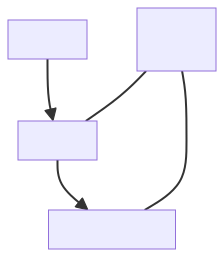
\includegraphics[keepaspectratio]{../../assets/organ_will_placement/attunement.png}}

}

\caption{調律の位置関係}

\end{figure}%

\begin{itemize}
\tightlist
\item
  意志はどこも操作しない
\item
  反応と行動の間に「間」を作る
\item
  反応 ≠ 行動 が可能になる
\end{itemize}

\subsection{状態}\label{ux72b6ux614b}

\begin{longtable}[]{@{}
  >{\raggedright\arraybackslash}p{(\linewidth - 10\tabcolsep) * \real{0.1667}}
  >{\raggedright\arraybackslash}p{(\linewidth - 10\tabcolsep) * \real{0.1667}}
  >{\raggedright\arraybackslash}p{(\linewidth - 10\tabcolsep) * \real{0.1667}}
  >{\raggedright\arraybackslash}p{(\linewidth - 10\tabcolsep) * \real{0.1667}}
  >{\raggedright\arraybackslash}p{(\linewidth - 10\tabcolsep) * \real{0.1667}}
  >{\raggedright\arraybackslash}p{(\linewidth - 10\tabcolsep) * \real{0.1667}}@{}}
\toprule\noalign{}
\begin{minipage}[b]{\linewidth}\raggedright
観点
\end{minipage} & \begin{minipage}[b]{\linewidth}\raggedright
調整
\end{minipage} & \begin{minipage}[b]{\linewidth}\raggedright
適応
\end{minipage} & \begin{minipage}[b]{\linewidth}\raggedright
適合
\end{minipage} & \begin{minipage}[b]{\linewidth}\raggedright
即興
\end{minipage} & \begin{minipage}[b]{\linewidth}\raggedright
調律
\end{minipage} \\
\midrule\noalign{}
\endhead
\bottomrule\noalign{}
\endlastfoot
\textbf{器官} & 使わない & 作動する(生理反射) & 作動する(免疫反応) &
作動する(衝動・表現) & 作動する(自己調節) \\
\textbf{意志の有無} & あり & なし & あり & あり & あり \\
\textbf{意志の位置} & 外部操作(行動・条件) & 不在 & 正当化(規範付与)
& 手放し & 間に留まる \\
\textbf{反応の性質} & 反応を無視 & 自動・閉 & 自動+固定 & 自発・開 &
感知のみ \\
\textbf{選択の有無} & 反応外で選択 & なし & 疑似的(正しさ依存) & あり
& あり \\
\textbf{停止可能性} & 高い & ない & 低い & あるが選ばない & ある \\
\textbf{境界の扱い} & 外部ルール & 生理的 & 規範的 & 不安定 &
構造的に保持 \\
\textbf{典型的な破綻} & 火消し依存 & 摩耗 & 排除・硬直 & 暴走 &
宙づり \\
\end{longtable}

適応 : 意志なし 即興 : 意志あり(流れる) 調律 : 意志あり(留まる)

\section{調律位置マップ}\label{ux8abfux5f8bux4f4dux7f6eux30deux30c3ux30d7}

\section{HAS
調律位置マップ}\label{has-ux8abfux5f8bux4f4dux7f6eux30deux30c3ux30d7}

HAS Attunement Map ― 状態の位置を知るための地図 ―

\subsection{この文書の位置づけ}\label{ux3053ux306eux6587ux66f8ux306eux4f4dux7f6eux3065ux3051}

この文書は、HASを\textbf{学ぶための段階表}ではない。\\
また、実践の巧拙を\textbf{評価する基準}でもない。

これは、\\
\textbf{いま自分がどこにいるかを誤解しないための地図}である。

HASにおいて重要なのは、

\begin{itemize}
\tightlist
\item
  進むことではなく
\item
  うまくやることでもなく
\item
  \textbf{選べる余地がなくなったときに、戻れること}
\end{itemize}

この地図は、そのために置かれている。

\begin{center}\rule{0.5\linewidth}{0.5pt}\end{center}

\subsection{基本原則}\label{ux57faux672cux539fux5247}

\subsubsection{この地図が示すもの}\label{ux3053ux306eux5730ux56f3ux304cux793aux3059ux3082ux306e}

この地図は、\textbf{状態(位置)のみ}を示す。

状態間の移動や戻り方(遷移)は、\\
\href{../resources/patterns/README.md}{Patterns} および
\href{../docs/08_failure_modes.md}{運用事故カタログ} に委ねられている。

\textbf{これは、位置を知ることと、動くことを分離するためである。}

\begin{figure}[H]

{\centering \pandocbounded{\includegraphics[keepaspectratio]{../assets/attunement_map.excalidraw.png}}

}

\caption{調律位置マップ}

\end{figure}%

\begin{verbatim}
[HAS外]
  └─(気づく)──────────────────────────▶ 観察

観察
  ├─(判断を保留する)──────────────────▶ 判断保留
  ├─(衝動・不安が増幅)────────────────▶ 乱れ
  └─(結論/完遂/介入固定)────────────▶ [HAS外]

判断保留
  ├─(試しに動く)────────────────────▶ 仮動
  ├─(戻ると判断)────────────────────▶ 観察
  ├─(耐えられなくなる)──────────────▶ 乱れ
  └─(結論/完遂/介入固定)────────────▶ [HAS外]

仮動
  ├─(試行を終える)──────────────────▶ 観察
  ├─(途中で止める)──────────────────▶ 判断保留
  ├─(制御不能)────────────────────▶ 乱れ
  └─(完遂目的化/操作化)────────────▶ [HAS外]

乱れ
  ├─(戻れると判断)──────────────────▶ 観察
  ├─(一段階戻る)──────────────────▶ 判断保留
  └─(操作・結論化)────────────────▶ [HAS外]
\end{verbatim}

\subsubsection{地図の読み方}\label{ux5730ux56f3ux306eux8aadux307fux65b9}

\begin{itemize}
\tightlist
\item
  ここに示されるのは「段階」ではなく\textbf{位置}である\\
\item
  上下・優劣・到達順序は存在しない\\
\item
  どの位置からでも、\textbf{観察に戻れる}
\end{itemize}

戻ることは後退ではない。\\
\textbf{戻れると判断できた時点で、HASは機能している。}

\subsubsection{HASが成立する前提条件}\label{hasux304cux6210ux7acbux3059ux308bux524dux63d0ux6761ux4ef6}

位置はすべて以下の前提の上に成り立つ:

\begin{itemize}
\tightlist
\item
  結論を確定していない(判断を閉じていない)
\item
  完遂を目的化していない
\item
  介入を「やるべきこと」として固定していない(操作モードになっていない)
\end{itemize}

これらの前提が満たされていない場合、その状態は HAS の外にある。

\begin{center}\rule{0.5\linewidth}{0.5pt}\end{center}

\subsection{HAS外の兆候(重要)}\label{hasux5916ux306eux5146ux5019ux91cdux8981}

以下のいずれかが起きている場合、現在の状態は \textbf{HAS の外}にある。

\begin{itemize}
\tightlist
\item
  結果を良くしようとして介入している
\item
  意味づけ・評価・結論を下している
\item
  完遂・成功・変化を目標に動いている
\item
  「正しくやれているか」を気にしている
\item
  \textbf{「この方法でいく」と手段を固定している(切り替え不能になっている)}
\end{itemize}

\subsubsection{HAS外にいる場合の対応}\label{hasux5916ux306bux3044ux308bux5834ux5408ux306eux5bfeux5fdc}

この場合、状態を特定しようとする前に、\\
\textbf{観察に戻る判断そのものが最初の実践となる。}

HAS外にいることは、失敗ではない。\\
気づいた時点で、観察に戻ればよい。

\begin{center}\rule{0.5\linewidth}{0.5pt}\end{center}

\subsection{4つの位置(States)}\label{ux3064ux306eux4f4dux7f6estates}

\subsubsection{観察(Observation)}\label{ux89b3ux5bdfobservation}

すべての実践は、ここから始まり、ここに戻る。

初心者も、経験者も区別されない。\\
ここは「準備段階」ではなく、\textbf{正規の位置}である。

\paragraph{内部定義}\label{ux5185ux90e8ux5b9aux7fa9}

刺激に対して生じつつある身体反応を、\\
意味づけや感情名を与えずに認知している状態。

判断はまだ立ち上がっていない。

\paragraph{この位置にいる兆候(Signs)}\label{ux3053ux306eux4f4dux7f6eux306bux3044ux308bux5146ux5019signs}

\begin{itemize}
\tightlist
\item
  身体の緊張や違和感に気づいている
\item
  衝動が立ち上がりつつあることを認知している
\item
  介入せず、判断が立ち上がる前に気づけている
\item
  呼吸が浅くなりすぎていない
\end{itemize}

\paragraph{観察における Patterns
との関係}\label{ux89b3ux5bdfux306bux304aux3051ux308b-patterns-ux3068ux306eux95a2ux4fc2}

観察にいるとき、P01--P04 はいずれも実行されない。\\
\textbf{それで HAS は成立している。}

\paragraph{注意}\label{ux6ce8ux610f}

\textbf{※HAS外条件}: 結論/完遂/介入固定が立ち上がったら HAS
外。観察へ戻る。

\begin{itemize}
\tightlist
\item
  何もしないことは放棄ではない\\
\item
  介入しない判断は、責任の放棄ではない\\
\item
  観察に留まることは、正規の実践である
\end{itemize}

\begin{center}\rule{0.5\linewidth}{0.5pt}\end{center}

\subsubsection{判断保留(Suspended
Judgment)}\label{ux5224ux65adux4fddux7559suspended-judgment}

この位置の目的は、良くすることではない。\\
\textbf{選択の余地が残っている位置に留まる}だけである。

\paragraph{内部定義}\label{ux5185ux90e8ux5b9aux7fa9-1}

観察の結果、起きていることや感じていることを、解釈前の``事実''として扱って受け取っているが、\\
その意味付けや解釈、次の行為に関する判断は宙吊りにされている状態。

選択の余地を奪わないため介入の制限が起きている。

\textbf{哲学的には、エポケー(判断中止)に相当する状態。}

\paragraph{この位置にいる兆候(Signs)}\label{ux3053ux306eux4f4dux7f6eux306bux3044ux308bux5146ux5019signs-1}

\begin{itemize}
\tightlist
\item
  介入したい衝動を抑えている
\item
  状態が整っていないことを「問題化」していない
\item
  場を進めようとしていない
\item
  「何もしていない」ことに焦りを感じていない
\end{itemize}

\paragraph{判断保留における Patterns
との関係}\label{ux5224ux65adux4fddux7559ux306bux304aux3051ux308b-patterns-ux3068ux306eux95a2ux4fc2}

判断保留では、P01 が自然に立ち上がることがあるが、\\
\textbf{それ以上進まなくてもよい。}

\paragraph{注意}\label{ux6ce8ux610f-1}

\textbf{※HAS外条件}: 結論/完遂/介入固定が立ち上がったら HAS
外。観察へ戻る。

\begin{itemize}
\tightlist
\item
  結果(良くなった/悪くなった)では判定しない\\
\item
  自己評価に使わない\\
\item
  事後評価も不要
\end{itemize}

\begin{center}\rule{0.5\linewidth}{0.5pt}\end{center}

\subsubsection{仮動(けどう / Tentative
Action)}\label{ux4eeeux52d5ux3051ux3069ux3046-tentative-action}

仮動とは、「一巡を完遂すること」ではない。\\
\textbf{進まないという判断を含んだ試行}である。

\paragraph{内部定義}\label{ux5185ux90e8ux5b9aux7fa9-2}

\textbf{仮動(けどう)}:
仮に動いてみること。本実行や完遂を目的としない試行的な行為状態。

P01から入り、試行的に動いているが、完遂を目指していない状態。\\
成果への期待も、評価の対象化もされていない。

\paragraph{この位置にいる兆候(Signs)}\label{ux3053ux306eux4f4dux7f6eux306bux3044ux308bux5146ux5019signs-2}

\begin{itemize}
\tightlist
\item
  P01 から入り、途中で止まっている
\item
  状態が変わらないことを失敗と見なしていない
\item
  「今はここまで」と判断できている
\item
  完遂への焦りがない
\end{itemize}

\paragraph{仮動における Pattern
との関係}\label{ux4eeeux52d5ux306bux304aux3051ux308b-pattern-ux3068ux306eux95a2ux4fc2}

仮動は、P01 から入り、途中で止まることを含む。\\
\textbf{P04 に至らなくても失敗ではない。}

\paragraph{仮動からの戻り(重要)}\label{ux4eeeux52d5ux304bux3089ux306eux623bux308aux91cdux8981}

仮動から観察へ戻ることは、失敗や乱れを意味しない。\\
試行を終え、再び気づきの位置に戻るという、\textbf{正常な遷移である。}

\paragraph{注意}\label{ux6ce8ux610f-2}

\textbf{※HAS外条件}: 結論/完遂/介入固定が立ち上がったら HAS
外。観察へ戻る。

\begin{itemize}
\tightlist
\item
  Pattern を道具として切り出さない\\
\item
  「P03 だけを使う」という発想を持たない\\
\item
  一部だけを「やろう」とした瞬間、断片化が始まる
\end{itemize}

\begin{center}\rule{0.5\linewidth}{0.5pt}\end{center}

\subsubsection{乱れ(みだれ /
Disruption)}\label{ux4e71ux308cux307fux3060ux308c-disruption}

HAS は、失敗しない体系ではない。\\
\textbf{戻れる体系}である。

乱れは、「失敗」ではなく、\textbf{位置}である。

\paragraph{内部定義}\label{ux5185ux90e8ux5b9aux7fa9-3}

主体または場の関係が乱れており、継続が難しい状態。

乱れは、必ず通過すべき関門ではない。\\
\textbf{破綻時・失敗時に現れる非常口}である。

\paragraph{この位置にいる兆候(Signs)}\label{ux3053ux306eux4f4dux7f6eux306bux3044ux308bux5146ux5019signs-3}

\begin{itemize}
\tightlist
\item
  自分または場の関係が乱れている
\item
  焦りが強い
\item
  介入衝動が抑えられない
\item
  沈黙に耐えられない
\item
  継続が難しいと感じている
\end{itemize}

\paragraph{乱れからの戻り}\label{ux4e71ux308cux304bux3089ux306eux623bux308a}

この位置から 観察 または 判断保留 に戻ることが、\\
\textbf{HAS の正常な動作である。}

戻る判断ができた時点で、乱れは機能している。

\paragraph{注意}\label{ux6ce8ux610f-3}

\textbf{※HAS外条件}: 結論/完遂/介入固定が立ち上がったら HAS
外。観察へ戻る。

\begin{itemize}
\tightlist
\item
  乱れを恥じない\\
\item
  戻りを正当化する必要はない\\
\item
  「いま戻る」と内的に判断すれば十分
\end{itemize}

\begin{center}\rule{0.5\linewidth}{0.5pt}\end{center}

\subsection{位置間の関係(図式)}\label{ux4f4dux7f6eux9593ux306eux95a2ux4fc2ux56f3ux5f0f}

\begin{verbatim}
観察 ⇄ 判断保留 ⇄ 仮動
 ↑  ↖─────────────↙  ↑
 │        乱れ        │
 └───────────────────┘
\end{verbatim}

\subsubsection{図の読み方}\label{ux56f3ux306eux8aadux307fux65b9}

\textbf{横の矢印(⇄)}: 通常・健全な遷移

\begin{itemize}
\tightlist
\item
  観察 ⇄ 判断保留
\item
  判断保留 ⇄ 仮動
\item
  仮動 → 観察(試行を終え、気づきに戻る)
\end{itemize}

\textbf{下のループ}: 乱れた場合の回復経路

\begin{itemize}
\tightlist
\item
  観察 → 乱れ → 観察
\item
  判断保留 → 乱れ → 判断保留 / 観察
\item
  仮動 → 乱れ → 判断保留 / 観察
\end{itemize}

乱れは「経由点」ではなく、\textbf{例外位置}である。

\begin{center}\rule{0.5\linewidth}{0.5pt}\end{center}

\subsubsection{遷移の詳細}\label{ux9077ux79fbux306eux8a73ux7d30}

遷移の方法は、以下を参照: -
\href{../resources/patterns/state/}{Patterns P01--P04} -
\href{./08_failure_modes.md}{運用事故カタログ} -
\href{../governance/protocols/emergency_stop.md}{Emergency Stop
Protocol}

\begin{center}\rule{0.5\linewidth}{0.5pt}\end{center}

\subsection{自己確認の問い}\label{ux81eaux5df1ux78baux8a8dux306eux554fux3044}

\subsubsection{1.
まず、HASの中にいるか確認する}\label{ux307eux305ahasux306eux4e2dux306bux3044ux308bux304bux78baux8a8dux3059ux308b}

以下のいずれかに該当する場合、HAS外にいる:

\begin{itemize}
\tightlist
\item
  結果を良くしようとしている
\item
  評価・結論を下している
\item
  完遂を目指している
\item
  「正しくやれているか」を気にしている
\item
  手段を固定している(切り替え不能になっている)
\end{itemize}

→ \textbf{観察に戻る}

\subsubsection{2.
HASの中にいる場合、位置を確認する}\label{hasux306eux4e2dux306bux3044ux308bux5834ux5408ux4f4dux7f6eux3092ux78baux8a8dux3059ux308b}

いま、私はどこにいるか?

\begin{enumerate}
\def\labelenumi{\arabic{enumi}.}
\tightlist
\item
  \textbf{何も介入していない} → 観察
\item
  \textbf{介入しないよう抑えている} → 判断保留
\item
  \textbf{進んでいるが完遂を目指していない} → 仮動
\item
  \textbf{乱れており、戻りたい} → 乱れ
\end{enumerate}

\subsubsection{重要な注意}\label{ux91cdux8981ux306aux6ce8ux610f}

\begin{itemize}
\tightlist
\item
  この問いは、\textbf{評価のためではない}
\item
  位置を知ることで、次の判断が可能になる
\item
  どの位置にいても、\textbf{観察}に戻れる
\end{itemize}

\begin{center}\rule{0.5\linewidth}{0.5pt}\end{center}

\subsection{慣れ親しむこと(熟練の再定義)}\label{ux6163ux308cux89aaux3057ux3080ux3053ux3068ux719fux7df4ux306eux518dux5b9aux7fa9}

HAS において、目指すのは熟練(Mastery)ではない。

目指すのは、\\
\textbf{この地図との関係に慣れ親しむこと(Familiarity)}である。

慣れ親しんだ者は、 - 迷わず\textbf{観察}に戻れる -
戻ることを失敗と解釈しない - 位置を誤解しない

それだけである。

\begin{center}\rule{0.5\linewidth}{0.5pt}\end{center}

\subsection{この地図の限界}\label{ux3053ux306eux5730ux56f3ux306eux9650ux754c}

\subsubsection{この地図が示さないもの}\label{ux3053ux306eux5730ux56f3ux304cux793aux3055ux306aux3044ux3082ux306e}

\begin{itemize}
\tightlist
\item
  遷移の方法(どう動くか)
\item
  Patterns の使い方(何をするか)
\item
  成果の評価(うまくいったか)
\end{itemize}

これらは、他の文書が担当する。

\subsubsection{この地図が示すもの}\label{ux3053ux306eux5730ux56f3ux304cux793aux3059ux3082ux306e-1}

\begin{itemize}
\tightlist
\item
  位置の識別(どこにいるか)
\item
  戻りの正当性(戻っていいか)
\item
  許可の範囲(やらなくていいこと)
\end{itemize}

\textbf{この地図は、動かすための設計書ではない。}\\
\textbf{迷子にならないための地図である。}

\begin{center}\rule{0.5\linewidth}{0.5pt}\end{center}

\subsection{関連文書}\label{ux95a2ux9023ux6587ux66f8-1}

\subsubsection{遷移と循環について}\label{ux9077ux79fbux3068ux5faaux74b0ux306bux3064ux3044ux3066}

\begin{itemize}
\tightlist
\item
  \href{./01_architecture_map.md}{全体設計図} --- HAS全体の構造
\item
  \href{../resources/patterns/state/}{Patterns P01--P04} ---
  状態遷移の構造
\end{itemize}

\subsubsection{位置の詳細について}\label{ux4f4dux7f6eux306eux8a73ux7d30ux306bux3064ux3044ux3066}

\begin{itemize}
\tightlist
\item
  \href{./03_principle.md}{判断優先原則} - 優先する判断の基準
\item
  \href{./05_facilitator_pitfalls.md}{ファシリテーターの落とし穴} -
  陥りやすい落とし穴
\item
  \href{./08_failure_modes.md}{運用事故カタログ} --- 乱れの典型
\end{itemize}

\subsubsection{緊急時の対応}\label{ux7dcaux6025ux6642ux306eux5bfeux5fdc}

\begin{itemize}
\tightlist
\item
  \href{../governance/protocols/emergency_stop.md}{Emergency Stop
  Protocol} --- 緊急停止の手続き
\end{itemize}

\begin{center}\rule{0.5\linewidth}{0.5pt}\end{center}

\textbf{この地図は、進むためのものではない。}\\
\textbf{選択の余地を狭めずに、居続けるためのものである。}

\begin{center}\rule{0.5\linewidth}{0.5pt}\end{center}

\subsection{Document Control}\label{document-control-2}

\begin{itemize}
\tightlist
\item
  \textbf{Repo Version:} v2.4.1-hotfix.1-1-ge4cc7141-dirty
\item
  \textbf{Last Modified:} 2025-12-26
\item
  \textbf{Commit:} fb73d68
\item
  \textbf{Author:} Takeshi Kakeda
\end{itemize}

\newpage

\section{実践編}\label{ux5b9fux8df5ux7de8}

\subsection{判断の優先指針}\label{ux5224ux65adux306eux512aux5148ux6307ux91dd}

\section{HAS
判断優先原則}\label{has-ux5224ux65adux512aux5148ux539fux5247}

\textbf{判断が割れたときの優先原則}

\subsection{この文書の役割}\label{ux3053ux306eux6587ux66f8ux306eux5f79ux5272}

この文書は、HASを実践・適用する際に、
\textbf{判断が割れたとき、どちらを優先するかを定める原則集}である。

これは: - 行動規範ではない - 倫理的理想像ではない -
強制される姿勢ではない

\textbf{介入・非介入、促進・待機など、境界上の判断を支えるための優先軸}である。

\begin{center}\rule{0.5\linewidth}{0.5pt}\end{center}

\subsection{原則}\label{ux539fux5247}

\subsubsection{原則1:
状態に正直であること}\label{ux539fux52471-ux72b6ux614bux306bux6b63ux76f4ux3067ux3042ux308bux3053ux3068}

\textbf{State over Performance}

迷ったら「成果」より「状態」を優先する。

整っていないなら、整っていないまま認める。\\
そこからしか始まらない。

\begin{center}\rule{0.5\linewidth}{0.5pt}\end{center}

\subsubsection{原則2:
恐れよりも、願いに耳を澄ますこと}\label{ux539fux52472-ux6050ux308cux3088ux308aux3082ux9858ux3044ux306bux8033ux3092ux6f84ux307eux3059ux3053ux3068}

\textbf{Want over Fear}

迷ったら「不安の解消」より「願いの識別」を優先する。

Mustと Fearの声は大きい。Wantはかすか。\\
かすかな方を聴く。

\begin{center}\rule{0.5\linewidth}{0.5pt}\end{center}

\subsubsection{原則3:
役割ではなく、人として向き合うこと}\label{ux539fux52473-ux5f79ux5272ux3067ux306fux306aux304fux4ebaux3068ux3057ux3066ux5411ux304dux5408ux3046ux3053ux3068}

\textbf{Being over Role}

迷ったら「役割の正しさ」より「存在の誠実さ」を優先する。

鎧は必要なときだけ着る。\\
常時装備すると、感情も関係も死ぬ。

\begin{center}\rule{0.5\linewidth}{0.5pt}\end{center}

\subsubsection{原則4:
違いを拒まず、響きとして受け取ること}\label{ux539fux52474-ux9055ux3044ux3092ux62d2ux307eux305aux97ffux304dux3068ux3057ux3066ux53d7ux3051ux53d6ux308bux3053ux3068}

\textbf{Resonance over Uniformity}

迷ったら「同質化」より「差異の保持」を優先する。

同質化は楽だが、知性を腐らせる。\\
差異があるから調律が生まれる。

\begin{center}\rule{0.5\linewidth}{0.5pt}\end{center}

\subsubsection{原則5:
速さではなく、整いから動くこと}\label{ux539fux52475-ux901fux3055ux3067ux306fux306aux304fux6574ux3044ux304bux3089ux52d5ux304fux3053ux3068}

\textbf{Readiness over Speed}

迷ったら「早く進む」より「整ってから動く」を優先する。

整っていない行動はただのノイズ。\\
整ってからでいい。

\begin{center}\rule{0.5\linewidth}{0.5pt}\end{center}

\subsubsection{原則6:
進むことと同じくらい、退くことを許すこと}\label{ux539fux52476-ux9032ux3080ux3053ux3068ux3068ux540cux3058ux304fux3089ux3044ux9000ux304fux3053ux3068ux3092ux8a31ux3059ux3053ux3068}

\textbf{Permission to Withdraw over Pressure}

迷ったら「前進」より「退却」を許す。

撤退は弱さではなく、回復の技法である。

\begin{center}\rule{0.5\linewidth}{0.5pt}\end{center}

\subsubsection{原則7:
本来のあり方に戻ることを、つねに選ぶこと}\label{ux539fux52477-ux672cux6765ux306eux3042ux308aux65b9ux306bux623bux308bux3053ux3068ux3092ux3064ux306dux306bux9078ux3076ux3053ux3068}

\textbf{Return over Achievement}

迷ったら「達成」より「回帰」を選ぶ。

Doingの前にBeing。\\
行動はいつも、状態の後を追う。

\begin{center}\rule{0.5\linewidth}{0.5pt}\end{center}

\subsection{落とし穴との関係}\label{ux843dux3068ux3057ux7a74ux3068ux306eux95a2ux4fc2}

\textbf{判断優先原則 と 落とし穴 は対をなす。}

\begin{itemize}
\tightlist
\item
  \textbf{判断優先原則:} どちらに進むかを決める(正の原則)
\item
  \textbf{落とし穴:} 行き過ぎを止める(負のガードレール)
\end{itemize}

この2つが揃って、初めて判断が安定する。

\begin{center}\rule{0.5\linewidth}{0.5pt}\end{center}

\subsection{使い方}\label{ux4f7fux3044ux65b9}

\subsubsection{ケース1:
沈黙が続いている}\label{ux30b1ux30fcux30b91-ux6c88ux9ed9ux304cux7d9aux3044ux3066ux3044ux308b}

\textbf{迷い:} 介入すべきか?待つべきか?

\textbf{判断優先原則による判断:} - 原則5「整いから動く」 →
整っていないなら、待つ

\textbf{落とし穴による検証:} - Failure Mode A「沈黙の美化」 →
苦痛の兆候があるなら、緊急停止を検討

\begin{center}\rule{0.5\linewidth}{0.5pt}\end{center}

\subsubsection{ケース2:
「正しい答え」を求められた}\label{ux30b1ux30fcux30b92-ux6b63ux3057ux3044ux7b54ux3048ux3092ux6c42ux3081ux3089ux308cux305f}

\textbf{迷い:} 答えるべきか?黙るべきか?

\textbf{判断優先原則による判断:} - 原則2「恐れより願い」 →
相手のFear(不安)に答えを与えても、Wantは満たされない

\textbf{落とし穴による検証:} - Failure Mode D「診断化」 →
「本当はこうしたいんでしょ?」と決めつけない

\begin{center}\rule{0.5\linewidth}{0.5pt}\end{center}

\subsubsection{ケース3:
参加者が苦しそう}\label{ux30b1ux30fcux30b93-ux53c2ux52a0ux8005ux304cux82e6ux3057ux305dux3046}

\textbf{迷い:} 助けるべきか?触れないべきか?

\textbf{判断優先原則による判断:} - 原則1「状態に正直」 →
自分が「助けたい焦り」から動いているなら、止まる

\textbf{落とし穴による検証:} - Failure Mode A「ネグレクト」 →
苦痛の兆候(震え、涙、虚ろな目)があるなら、緊急停止

\begin{center}\rule{0.5\linewidth}{0.5pt}\end{center}

\subsection{関連文書}\label{ux95a2ux9023ux6587ux66f8-2}

\begin{itemize}
\tightlist
\item
  \href{./00_manifesto.md}{マニフェスト} --- 守るもの
\item
  \href{./05_facilitator_pitfalls.md}{ファシリテーターの落とし穴} ---
  事故カタログ
\item
  \href{./08_failure_modes.md}{運用事故カタログ} --- 詳細な失敗パターン
\item
  \href{../core/HAS_v2.0_Final.md}{HASカーネル} --- 憲法と禁忌
\end{itemize}

\begin{center}\rule{0.5\linewidth}{0.5pt}\end{center}

\subsection{Document Control}\label{document-control-3}

\begin{itemize}
\tightlist
\item
  \textbf{Repo Version:} v2.4.1-hotfix.1-1-ge4cc7141-dirty
\item
  \textbf{Last Modified:} 2025-12-26
\item
  \textbf{Commit:} fb73d68
\item
  \textbf{Author:} Takeshi Kakeda
\end{itemize}

\newpage

\subsection{陥りやすい落とし穴}\label{ux9665ux308aux3084ux3059ux3044ux843dux3068ux3057ux7a74}

\section{ファシリテーターの落とし穴}\label{ux30d5ux30a1ux30b7ux30eaux30c6ux30fcux30bfux30fcux306eux843dux3068ux3057ux7a74}

\textbf{Facilitator Pitfalls}

\begin{center}\rule{0.5\linewidth}{0.5pt}\end{center}

\subsection{このドキュメントの位置づけ}\label{ux3053ux306eux30c9ux30adux30e5ux30e1ux30f3ux30c8ux306eux4f4dux7f6eux3065ux3051}

この文書は、HASの実践において\\
\textbf{ファシリテーター自身が陥りやすい構造}を記述する。

これは規範ではない。\\
守るべき原則でもない。\\
\textbf{選択の余地が失われていく過程の地図}である。

\begin{center}\rule{0.5\linewidth}{0.5pt}\end{center}

\subsection{前提:ファシリテーターは場の一部である}\label{ux524dux63d0ux30d5ux30a1ux30b7ux30eaux30c6ux30fcux30bfux30fcux306fux5834ux306eux4e00ux90e8ux3067ux3042ux308b}

HASにおいて、ファシリテーターと場は分離できない。

\begin{itemize}
\tightlist
\item
  場を「観察する主体」として外側に立つことはできない
\item
  ファシリテーター自身の状態が、場の状態に影響を及ぼす
\item
  この影響は意図ではなく、\textbf{存在(Presence)として現れる}
\end{itemize}

この前提を忘れた瞬間、HASは操作に転じる。

※本文書では、「介入」という語を避け、「影響」「関与」「Presence」を用いる。

\begin{center}\rule{0.5\linewidth}{0.5pt}\end{center}

\subsection{陥りやすいポイント}\label{ux9665ux308aux3084ux3059ux3044ux30ddux30a4ux30f3ux30c8}

以下は、ファシリテーターが陥りやすい構造である。\\
これらに気づいたら、\textbf{観察(何もしない)に戻ることが適切}である。

\subsubsection{1.
自己の状態を観ずに関与する}\label{ux81eaux5df1ux306eux72b6ux614bux3092ux89b3ux305aux306bux95a2ux4e0eux3059ux308b}

\textbf{兆候:} -
焦り・緊張・「何とかしなければ」が出ているまま動いている -
沈黙を埋めたい衝動が強い - 相手を「変えたい」「良くしたい」欲が出ている

\textbf{結果:} 場の緊張が増幅され、参加者の選択肢が狭まる

\textbf{戻り方:} 観察(何もしない)に退避する。\\
何もしないことは、放棄ではなく判断である。

詳細:\href{./08_failure_modes.md\#failure-mode-g-facilitatorの状態無視}{Failure
Mode G: Facilitatorの状態無視}

\begin{center}\rule{0.5\linewidth}{0.5pt}\end{center}

\subsubsection{2.
沈黙を「問題」として扱う}\label{ux6c88ux9ed9ux3092ux554fux984cux3068ux3057ux3066ux6271ux3046}

\textbf{兆候:} - 沈黙が続くと不安になり、何か言わなければと感じる -
「難しいですよね」「例えば\ldots」と沈黙を埋めようとする -
沈黙の時間をカウントし、「十分待った」と判断しようとする

\textbf{結果:}
参加者の内省プロセスが中断され、借り物の言葉しか出なくなる

\textbf{戻り方:} P03の原則を想起する。\\
沈黙は「空白」ではなく「充満」である。

\textbf{⚠️ 重要な境界:}\\
沈黙は「安全の代替」ではない。\\
苦痛・危機の兆候がある場合は、HAS Kernelの緊急停止を優先する。

詳細:\href{./08_failure_modes.md\#failure-mode-a-沈黙の美化によるネグレクト}{Failure
Mode A: 沈黙の美化によるネグレクト}

\begin{center}\rule{0.5\linewidth}{0.5pt}\end{center}

\subsubsection{3.
完璧主義ループ}\label{ux5b8cux74a7ux4e3bux7fa9ux30ebux30fcux30d7}

\textbf{兆候:} - 「私はまだ整っていない」と永遠に自己否定する -
または「私は整っている」という自己欺瞞で防衛する -
観察に戻ることを「失敗」として内面化している

\textbf{結果:} 実践そのものが停止する。燃え尽き、自己否定の深化。

\textbf{戻り方:} 観察は正規の実践であると認識する。\\
何もしないことは、最も誠実な判断である。

詳細:\href{./08_failure_modes.md\#failure-mode-e-完璧主義ループ自己監視の宗教化}{Failure
Mode E: 完璧主義ループ}

\begin{center}\rule{0.5\linewidth}{0.5pt}\end{center}

\subsubsection{4.
Fear/Want判定を相手に告げる}\label{fearwantux5224ux5b9aux3092ux76f8ux624bux306bux544aux3052ux308b}

\textbf{兆候:} - 「あなたは今、恐れから話している」と指摘する -
「それは本音じゃないよね」と誘導する -
「Wantが出ない」ことを問題視し、引き出そうとする

\textbf{結果:}
診断される侵襲体験。分析者vs被分析者という非対称の固定化。

\textbf{戻り方:} P02の原則を再確認する。\\
区別は内的操作に留める。告げない。

詳細:\href{./08_failure_modes.md\#failure-mode-d-fearwant判定の投影診断化}{Failure
Mode D: Fear/Want判定の投影・診断化}

\begin{center}\rule{0.5\linewidth}{0.5pt}\end{center}

\subsection{観察への退避は常に可能}\label{ux89b3ux5bdfux3078ux306eux9000ux907fux306fux5e38ux306bux53efux80fd}

整っていない状態を認識した時、\\
\textbf{観察(何もしない)は常に選択可能である。}

これは失敗ではない。\\
責任放棄でもない。\\
\textbf{最も誠実な判断}である。

観察について詳しくは:\href{./04_attunement_map.md\#観察(Observation)}{調律位置マップ}

\begin{center}\rule{0.5\linewidth}{0.5pt}\end{center}

\subsection{関連文書}\label{ux95a2ux9023ux6587ux66f8-3}

\begin{itemize}
\tightlist
\item
  \href{./04_attunement_map.md}{調律位置マップ} --- Level 0の詳細
\item
  \href{./08_failure_modes.md}{運用事故カタログ} --- 事故モード
\item
  \href{../resources/patterns/state/}{P01-P04 Patterns} ---
  各パタンのFacilitator Self-Check
\item
  \href{../core/HAS_v2.0_Final.md}{HAS Kernel} --- 非介入の定義
\item
  \href{../governance/protocols/emergency_stop.md}{Emergency Stop
  Protocol} --- 緊急停止の判断基準
\end{itemize}

\begin{center}\rule{0.5\linewidth}{0.5pt}\end{center}

\subsection{Document Control}\label{document-control-4}

\begin{itemize}
\tightlist
\item
  \textbf{Repo Version:} v2.4.1-hotfix.1-1-ge4cc7141
\item
  \textbf{Last Modified:} 2025-12-26
\item
  \textbf{Commit:} fb73d68
\item
  \textbf{Author:} Takeshi Kakeda
\end{itemize}

\newpage

\subsection{状態パタン}\label{ux72b6ux614bux30d1ux30bfux30f3}

\section{状態パタン}\label{ux72b6ux614bux30d1ux30bfux30f3-1}

― 状態を「やっていること」ではなく「見えている様子」として捉える ―

\subsection{この文書の目的}\label{ux3053ux306eux6587ux66f8ux306eux76eeux7684}

この文書は、状態パタン(P01--P04)を実践手順や内面理解として説明しない。

ここで扱うのは、\textbf{場や人に「どう見えるか」「どんな雰囲気として現れるか」}という外観のみ。

\begin{itemize}
\tightlist
\item
  良し悪しを判定しない
\item
  正しい使い方を示さない
\item
  次に何をすべきかは決めない
\end{itemize}

「今、どの状態に``見えるか''」を誤認しないための補助資料である。

⸻

\begin{figure}[H]

{\centering \pandocbounded{\includegraphics[keepaspectratio]{../../../assets/state_patterns.png}}

}

\caption{状態パタンの遷移図}

\end{figure}%

状態パタンは「行為」ではなく「様相」

HASにおける状態パタンは、誰かが何かを「している」状態ではない。

\begin{itemize}
\tightlist
\item
  技法が使われているかどうかではない
\item
  ファシリテーターの意図でもない
\item
  発言内容の正しさでもない
\end{itemize}

結果として、場に立ち現れている様相である。

したがって、同じ発言でも、状態が違えば外観は異なる。

\newpage

\subsection{状態パタン01
置かれた感情}\label{ux72b6ux614bux30d1ux30bfux30f301-ux7f6eux304bux308cux305fux611fux60c5}

\section{P01:
置かれた感情}\label{p01-ux7f6eux304bux308cux305fux611fux60c5}

\textbf{Placed Emotion}

\textbf{感情を花瓶のように置く}

\begin{center}\rule{0.5\linewidth}{0.5pt}\end{center}

\subsection{Context}\label{context}

\begin{itemize}
\tightlist
\item
  会話は進んでいるが、場に緊張や硬さがある
\item
  建設的・前向きな発言だけが流通している
\item
  違和感や不満が「言わない方がいいもの」になっている
\item
  感情が議題の外に追い出されている
\end{itemize}

\begin{center}\rule{0.5\linewidth}{0.5pt}\end{center}

\subsection{Forces}\label{forces}

\subsubsection{Pressure (圧力)}\label{pressure-ux5727ux529b}

感情という「非効率なノイズ」を、場から排除しようとする不可視の力学。

\begin{itemize}
\tightlist
\item
  \textbf{効率性への圧力:}
  「生産的でなければならない」「早く整えたい」という無言の焦燥感。
\item
  \textbf{同調への圧力:}
  「前向きであるべきだ」という空気感による無意識の強制。
\end{itemize}

\subsubsection{Fear (恐れ)}\label{fear-ux6050ux308c}

個人的な感情を場に出すことが、平穏な進行を妨げる「異物」となることへの恐怖。

\begin{itemize}
\tightlist
\item
  \textbf{場の崩壊への恐れ:}
  感情を出すことで、今の平穏な(しかし硬直した)空気が壊れることへの恐怖。
\item
  \textbf{異物になる恐れ:}
  自分の弱さを見せることで、進行を妨げる「異物」として扱われることへの恐怖。
\end{itemize}

\subsubsection{Armor (防衛)}\label{armor-ux9632ux885b}

生の感情を「処理可能な情報」へと変換し、無害化しようとする無意識の防衛。

\begin{itemize}
\item
  \textbf{知性化:} 冷静さ・合理性という鎧で、感情の揺らぎを覆い隠す。
\item
  \textbf{一般化:} 冗談や一般論に逃げ込み、個人的な痛点に触れさせない。
\item
  \textbf{課題化:}
  「結局どうしたい?」と問いかけ、感情を即座に論理的課題へと変換し、無害化する。
\item
  \begin{center}\rule{0.5\linewidth}{0.5pt}\end{center}
\end{itemize}

\subsection{Problem}\label{problem}

感情が「処理すべきノイズ」として扱われ、
場は静かだが、内側の緊張は残り続ける。
\textbf{ここでは「わかろうとする(共感)」こと自体が、関与の圧になる。}

\begin{center}\rule{0.5\linewidth}{0.5pt}\end{center}

\subsection{Essence}\label{essence}

感情を「解決すべき課題」としてではなく、
\textbf{「テーブルの上の花瓶」のように扱う。}

ただ、そこに在ることを認める(\textbf{置く})。
しかし、その花を生け直したり、分析したりはしない(\textbf{通過させる})。

\begin{itemize}
\tightlist
\item
  名前をつけなくていい(ラベリングしない)
\item
  要約しなくていい(まとめない)
\item
  意味づけなくていい(解釈しない)
\end{itemize}

\textbf{「あぁ、今ここに赤い花(怒り)があるな」と眺めるだけにする。}
手にとっていじくり回さないこと。

冷たく見えるかもしれないが、
\textbf{触らないことこそが、個人の領域を侵さない最大の敬意である。}

\begin{center}\rule{0.5\linewidth}{0.5pt}\end{center}

\subsection{Resulting Context}\label{resulting-context}

\begin{itemize}
\tightlist
\item
  感情が「私」という人格から切り離され(Defusion)、客観的な\textbf{現象}としてテーブルに置かれる
\item
  「いじられない(評価・介入されない)」という安心感から、知性化の防衛(Armor)が緩む
\item
  置かれた感情は、誰にも操作されず、やがて自然に流れていく
\end{itemize}

整わない限り、次の調律には進まない。

\begin{center}\rule{0.5\linewidth}{0.5pt}\end{center}

\subsection{Breakdown}\label{breakdown}

\begin{itemize}
\tightlist
\item
  「前向きさ」が同調圧力(Pressure)となる
\item
  「つまり〇〇ってこと?」とファシリテーターが解釈・要約を始め、Armorを強化してしまう
\item
  感情を表明すること自体が、新たな「ねばならない(Must)」という義務になる
\end{itemize}

\begin{center}\rule{0.5\linewidth}{0.5pt}\end{center}

\subsection{Facilitator Self-Check}\label{facilitator-self-check}

\begin{quote}
\textbf{⚠️ P01 Specific Trap:}
今、テーブルに置かれた花(感情)を、勝手に生け直そうとしていないか?
その「整えてあげたい善意」が、ここでは最大のノイズになる。
\end{quote}

\begin{center}\rule{0.5\linewidth}{0.5pt}\end{center}

\subsection{Minimal Actions}\label{minimal-actions}

\textbf{State を保つために許されている、最小限の動作。}
これ以上は介入になり、これ以下は放置になる。

\subsubsection{1. 宣言する
(Declare)}\label{ux5ba3ux8a00ux3059ux308b-declare}

\begin{itemize}
\tightlist
\item
  「解決しなくていい」「一言だけ置く」というルールを告げる。
\item
  \textbf{Script:}
  「今の天気を一言だけ置いてください。それに対して誰もコメントしません。」
\end{itemize}

\subsubsection{2. そのまま返す
(Echo)}\label{ux305dux306eux307eux307eux8fd4ux3059-echo}

\begin{itemize}
\tightlist
\item
  相手の言葉を変えずに、点(。)で止めて返す。
\item
  \textbf{OK:} 「イライラしているんですね。(沈黙)」
\item
  \textbf{NG:} 「進まなくてイライラしているんですね(解釈)」
\end{itemize}

\subsubsection{3. 眺める (Watch)}\label{ux773aux3081ux308b-watch}

\begin{itemize}
\tightlist
\item
  出てきた感情(言葉や付箋)を、数秒間ただ無言で眺める時間を取る。
\item
  すぐに「次は?」と進めない。
\end{itemize}

\begin{quote}
\textbf{Rule:} Minimal Actions
は、少ないほどよい。迷ったら「何もしない」を選ぶ。
\end{quote}

\begin{center}\rule{0.5\linewidth}{0.5pt}\end{center}

\subsection{Signals}\label{signals}

\begin{itemize}
\tightlist
\item
  沈黙中も呼吸が乱れない
\item
  割り込みが起きない
\item
  発話が短く、要点を突く(物語化しない)
\end{itemize}

\begin{center}\rule{0.5\linewidth}{0.5pt}\end{center}

\subsection{Document Control}\label{document-control-5}

\begin{itemize}
\tightlist
\item
  Pattern ID: P01 ~
\item
  Version: 1.7.0 ~
\item
  Date: 2025-12-13
\end{itemize}

\newpage

\subsection{状態パタン02
識別された感情}\label{ux72b6ux614bux30d1ux30bfux30f302-ux8b58ux5225ux3055ux308cux305fux611fux60c5}

\section{P02:
識別された感情}\label{p02-ux8b58ux5225ux3055ux308cux305fux611fux60c5}

\textbf{Differentiated Emotion}

\textbf{評価せず、決めず、区別されている状態}

\begin{center}\rule{0.5\linewidth}{0.5pt}\end{center}

\subsection{Context}\label{context-1}

\begin{itemize}
\tightlist
\item
  \textbf{P01:
  \href{./P01_placed_emotion.md}{置かれた感情}}により感情は落ち着いている
\item
  次に何をするかを急ぎ始めている
\item
  正しさ・合理性の議論が強まり始めている
\end{itemize}

\begin{center}\rule{0.5\linewidth}{0.5pt}\end{center}

\subsubsection{Pressure (圧力)}\label{pressure-ux5727ux529b-1}

場の空気を支配している不可視の力学。評価ではなく、現象として記述される。

\begin{itemize}
\tightlist
\item
  \textbf{正解への圧力:}
  「最適解以外は排除される」「論理的な隙は攻撃対象となる」という、場にかかる強い淘汰圧。
\item
  \textbf{合意への圧力:}
  「異論はノイズである」「早く一枚岩にならなければ進めない」という、同調への強力な引力。
\end{itemize}

\subsubsection{Fear (恐れ)}\label{fear-ux6050ux308c-1}

個人の内側で起きている、選択に対する根源的な震え。

\begin{itemize}
\tightlist
\item
  \textbf{孤立への恐れ:}
  自分の言葉で語り、自分で選ぶことは、集団から浮き上がり「一人」になることへの恐怖。
\item
  \textbf{否定への恐れ:}
  自分の提案が否定されることが、自分自身の存在や関係性そのものが拒絶される予兆として感じられる恐怖。
\item
  \textbf{不可逆への恐れ:}
  決定することによって他の可能性が死に、その結果責任を一人で引き受けることへの恐怖。
\end{itemize}

\subsubsection{Armor (防衛)}\label{armor-ux9632ux885b-1}

恐れを感じないために身につける、観測可能な振る舞い。

\begin{itemize}
\item
  \textbf{主語の隠蔽:}
  「私たちは」「普通は」と大きな主語や一般論で語り、自分の輪郭を消すことで責任の所在を曖昧にする。
\item
  \textbf{分析と評価:}
  他者の発言の背景を分析したり、是非を裁定したりすることで、自分が安全な「観察者」の立場に逃げ込む。
\item ~
  \subsection{\texorpdfstring{\textbf{即時構造化:}
  曖昧な願いや揺らぎを、即座に「目標・KPI・アクションプラン」という硬い構造に変換する。これは、情緒的な不確実性に耐えられないため、選択を先送りせずに固定化しようとする防衛である。}{即時構造化: 曖昧な願いや揺らぎを、即座に「目標・KPI・アクションプラン」という硬い構造に変換する。これは、情緒的な不確実性に耐えられないため、選択を先送りせずに固定化しようとする防衛である。}}\label{ux5373ux6642ux69cbux9020ux5316-ux66d6ux6627ux306aux9858ux3044ux3084ux63faux3089ux304eux3092ux5373ux5ea7ux306bux76eeux6a19kpiux30a2ux30afux30b7ux30e7ux30f3ux30d7ux30e9ux30f3ux3068ux3044ux3046ux786cux3044ux69cbux9020ux306bux5909ux63dbux3059ux308bux3053ux308cux306fux60c5ux7dd2ux7684ux306aux4e0dux78baux5b9fux6027ux306bux8010ux3048ux3089ux308cux306aux3044ux305fux3081ux9078ux629eux3092ux5148ux9001ux308aux305bux305aux306bux56faux5b9aux5316ux3057ux3088ux3046ux3068ux3059ux308bux9632ux885bux3067ux3042ux308b}
\end{itemize}

\subsection{Problem}\label{problem-1}

恐れから出た声が「願いのふり」をし、 本当に大切な Want が見えなくなる。

\begin{center}\rule{0.5\linewidth}{0.5pt}\end{center}

\subsection{Essence}\label{essence-1}

決めない。評価しない。 ただ \textbf{区別する}。

これは恐れか? それとも願いか?

判断基準は論理ではなく、\textbf{その場に現れる身体反応}。
恐れは「速く・硬く」、願いは「遅く・柔らかい」。

その違いを、\textbf{暴かず、指摘せず、ただ自分の中で見分ける。}

\begin{center}\rule{0.5\linewidth}{0.5pt}\end{center}

\subsection{Resulting Context}\label{resulting-context-1}

\begin{itemize}
\tightlist
\item
  表層的な合意が減る
\item
  自己正当化が静まる
\item
  本当に大切な Want だけが残る
\end{itemize}

Want が出てこなくても失敗ではない。

\begin{center}\rule{0.5\linewidth}{0.5pt}\end{center}

\subsection{Breakdown}\label{breakdown-1}

\begin{itemize}
\tightlist
\item
  「それは本当の Want?」と詰問(尋問)が始まる
\item
  Want が正解扱いされる
\item
  願いが即座に計画に変換される
\end{itemize}

\begin{center}\rule{0.5\linewidth}{0.5pt}\end{center}

\subsection{Facilitator Self-Check}\label{facilitator-self-check-1}

\begin{quote}
\textbf{⚠️ P02 Specific Trap:}
今、あなたは「本音ハンター(真実の尋問官)」になっていないか?
恐れ(Fear)を指摘して論破しようとしたり、願い(Want)を無理やり引き出そうとしていないか?
\end{quote}

\begin{center}\rule{0.5\linewidth}{0.5pt}\end{center}

\subsection{Minimal Actions}\label{minimal-actions-1}

\textbf{State を保つために許されている、最小限の動作。}
これ以上は介入になり、これ以下は放置になる。

\subsubsection{1. 問いを体に置く (Ask the
Body)}\label{ux554fux3044ux3092ux4f53ux306bux7f6eux304f-ask-the-body}

\begin{itemize}
\tightlist
\item
  内容(Logic)ではなく、身体反応(Somatic)について問う。
\item
  \textbf{Script:} 「それを言った時、体は重いですか?
  軽いですか?」「呼吸は楽ですか?」
\end{itemize}

\subsubsection{2. 内的に区別する (Internal
Distinguish)}\label{ux5185ux7684ux306bux533aux5225ux3059ux308b-internal-distinguish}

\begin{itemize}
\tightlist
\item
  ファシリテーター自身の中で「今のはFear(早口・防衛)だな」「今のはWant(遅い・探索)だな」と区別する。
\item
  \textbf{Rule:}
  それを相手に告げる必要はない。「それはFearですね」という指摘は、新たなFearを生む。
\item
  \textbf{参加者同士による同様の指摘も、同じく止める。}
\end{itemize}

\subsubsection{3. 待つ (Wait for the
Shift)}\label{ux5f85ux3064-wait-for-the-shift}

\begin{itemize}
\tightlist
\item
  Want特有の「遅い声」「沈黙」「言い淀み」が出るまで、口を挟まずに待つ。
\item
  整った言葉(Fear/Armor)には反応せず、崩れた言葉(Want)を拾う。
\end{itemize}

\begin{center}\rule{0.5\linewidth}{0.5pt}\end{center}

\subsection{Signals}\label{signals-1}

\begin{itemize}
\tightlist
\item
  Want が語られると声が遅くなる
\item
  一時的な沈黙が増える
\item
  断定語が減る
\end{itemize}

\begin{center}\rule{0.5\linewidth}{0.5pt}\end{center}

\subsection{Document Control}\label{document-control-6}

\begin{itemize}
\tightlist
\item
  Pattern ID: P02\\
\item
  Version: 1.2.0\\
\item
  Date: 2025-12-12
\end{itemize}

\newpage

\subsection{状態パタン03
不快への滞留}\label{ux72b6ux614bux30d1ux30bfux30f303-ux4e0dux5febux3078ux306eux6edeux7559}

\section{Pattern 03:
不快への滞留}\label{pattern-03-ux4e0dux5febux3078ux306eux6edeux7559}

\textbf{Lingering toward Discomfort}

\begin{quote}
不快にとどまり「空白」として処理されない状態を保つパタン。
\end{quote}

\begin{center}\rule{0.5\linewidth}{0.5pt}\end{center}

\subsection{Context}\label{context-2}

\begin{itemize}
\tightlist
\item
  \textbf{P02: \href{./P02_differentiated_emotion.md}{識別された感情}}
  を経て、まだ何かがひっかかっている。
\item
  まだ言葉・判断・行為に移れないが、しかしまだ逃げてもいない。
\item
  会議の場などで、その状態が沈黙として現れることがある。
\end{itemize}

\begin{center}\rule{0.5\linewidth}{0.5pt}\end{center}

\subsection{Forces}\label{forces-1}

\subsubsection{Pressure (圧力)}\label{pressure-ux5727ux529b-2}

ファシリテーターや参加者を、内側から「行為(Doing)」へと突き動かす不可視の重力。

\begin{itemize}
\tightlist
\item
  \textbf{進行への引力:}
  沈黙が続くほど、場の時間が停止しているように感じられ、一刻も早く「何かを動かさなければ」と身体を急き立てる引力。
\item
  \textbf{役割への引力:}
  「何もしていない」状態に耐えられず、何かしらの言葉を発して「ファシリテーター(または参加者)としての役割」を再確認しようとする引力。
\end{itemize}

\subsubsection{Fear (恐れ)}\label{fear-ux6050ux308c-2}

沈黙の中で、役割や意味が剥がれ落ちていくことに対する根源的な震え。

\begin{itemize}
\tightlist
\item
  \textbf{空虚への恐れ:}
  沈黙を「何も起きていない空白」と誤認し、その空虚さに自分や関係性が飲み込まれてしまうことへの恐怖。
\item
  \textbf{融解への恐れ:}
  役割(進行役、発言者)を手放し、ただそこに「存在しているだけ」の状態になることで、自分という輪郭が溶けてしまう感覚に対する恐怖。
\end{itemize}

\subsubsection{Armor (防衛)}\label{armor-ux9632ux885b-2}

不快感から逃れるために行われる、無意識の介入行動。

\begin{itemize}
\item
  \textbf{代理言語化:}
  「つまり、こういうことですか?」と、相手が言葉を探している最中に先回りして言語化し、沈黙を埋める。
\item
  \textbf{難易度調整:}
  「難しい質問でしたね」「例えば\ldots」と、答えやすい浅い問いを投げ直し、思考の深さをリセットする。
\item ~
  \subsection{\texorpdfstring{\textbf{自己投入:}
  自分の経験談や意見を語り始めることで、場の焦点を「参加者の内面」から「ファシリテーターの話題」へとそらす。}{自己投入: 自分の経験談や意見を語り始めることで、場の焦点を「参加者の内面」から「ファシリテーターの話題」へとそらす。}}\label{ux81eaux5df1ux6295ux5165-ux81eaux5206ux306eux7d4cux9a13ux8ac7ux3084ux610fux898bux3092ux8a9eux308aux59cbux3081ux308bux3053ux3068ux3067ux5834ux306eux7126ux70b9ux3092ux53c2ux52a0ux8005ux306eux5185ux9762ux304bux3089ux30d5ux30a1ux30b7ux30eaux30c6ux30fcux30bfux30fcux306eux8a71ux984cux3078ux3068ux305dux3089ux3059}
\end{itemize}

\subsection{Problem}\label{problem-2}

\textbf{沈黙のような不快が訪れた瞬間に介入することで、当事者が内側で起きているプロセスが自然に展開する余地を奪ってしまう。}

最も重要な「内省のプロセス」が、不安の回避行動によって中断される。

\begin{center}\rule{0.5\linewidth}{0.5pt}\end{center}

\subsection{Essence}\label{essence-2}

不快を処理しない。意味づけしない。突破しない。

不快が「対象」になる前の位置で、主体と不快の関係が切れないまま、動きが止まっている状態。

沈黙は、その状態が場に現れた一つの表れにすぎない。

\begin{center}\rule{0.5\linewidth}{0.5pt}\end{center}

\subsection{Resulting Context}\label{resulting-context-2}

\begin{itemize}
\tightlist
\item
  借り物ではない、重みのある言葉(Primary Words)が紡がれる
\item
  参加者全員が、発話者だけでなく「場そのもの」に耳を澄ませるようになる
\item
  \textbf{P04: 引受の成立} へと接続される土壌が整う
\end{itemize}

\begin{center}\rule{0.5\linewidth}{0.5pt}\end{center}

\subsection{Breakdown (Anti-Pattern)}\label{breakdown-anti-pattern}

\begin{itemize}
\tightlist
\item
  \textbf{助け舟:} 誰かが苦しそうに見えた瞬間、助け舟を出してしまう
\item
  \textbf{ラベリング:}
  「難しいですよね」と沈黙をネガティブに意味づけしてしまう
\end{itemize}

\begin{center}\rule{0.5\linewidth}{0.5pt}\end{center}

\subsection{Facilitator Self-Check}\label{facilitator-self-check-2}

\begin{quote}
私の呼吸は浅くなっていないか?
今、この沈黙を「解決」しようとしていないか?
\end{quote}

\begin{center}\rule{0.5\linewidth}{0.5pt}\end{center}

\subsection{Minimal Actions}\label{minimal-actions-2}

\textbf{沈黙を壊さず、State を保つために許されている最小動作。}
これ以上は介入になり、これ以下は逃避になる。

\subsubsection{1. 呼吸に留まる (Stay with
Breath)}\label{ux547cux5438ux306bux7559ux307eux308b-stay-with-breath}

\begin{itemize}
\tightlist
\item
  自分の呼吸だけを感じる。
\item
  言葉を探さない。問いを作らない。
\end{itemize}

\subsubsection{2. 視線を固定しない (Soften the
Gaze)}\label{ux8996ux7ddaux3092ux56faux5b9aux3057ux306aux3044-soften-the-gaze}

\begin{itemize}
\tightlist
\item
  特定の誰かを見つめない。
\item
  場全体、もしくは一点(テーブル・床)を見る。
\end{itemize}

\subsubsection{3. 沈黙を「切らない」 (Do Not
Cut)}\label{ux6c88ux9ed9ux3092ux5207ux3089ux306aux3044-do-not-cut}

\begin{itemize}
\tightlist
\item
  5秒、10秒、20秒というカウントをしない。
\item
  「十分待った」という判断をしない。
\end{itemize}

「何かをしよう」と気づいたら、\textbf{それをしない}。
これは我慢ではなく、\textbf{状態を壊さないための判断}である。

\begin{quote}
\textbf{Rule:} 沈黙が破られる「正しいタイミング」は存在しない。
破られたときが、そのタイミングである。
\end{quote}

\begin{center}\rule{0.5\linewidth}{0.5pt}\end{center}

\subsection{Signals}\label{signals-2}

\begin{itemize}
\tightlist
\item
  ファシリテーターの視線が柔らかく、一点に定まっている
\item
  参加者の視線が宙を漂うか、内側に向いている(誰も他者の顔色を窺っていない)
\item
  沈黙が破られた後、すぐに反応(相槌や同意)が起きず、再び静寂が戻る
\end{itemize}

\newpage

\subsection{状態パタン04
引受の成立}\label{ux72b6ux614bux30d1ux30bfux30f304-ux5f15ux53d7ux306eux6210ux7acb}

\section{Pattern 04:
引受の成立}\label{pattern-04-ux5f15ux53d7ux306eux6210ux7acb}

\textbf{Establishment of Ownership}

\begin{quote}
「不快への滞留」が熟し、内側から言葉が溢れ出るタイミングで使う。
\end{quote}

\begin{center}\rule{0.5\linewidth}{0.5pt}\end{center}

\subsection{Context}\label{context-3}

\begin{itemize}
\tightlist
\item
  \textbf{P03:
  \href{./P03_lingering_toward_discomfort.md}{不快への滞留}}
  を経て、場には十分に重たい「何か」が漂っている。
\item
  誰かが口火を切ろうとしているが、まだその言葉は宙に浮いており、着地していない。
\end{itemize}

\begin{center}\rule{0.5\linewidth}{0.5pt}\end{center}

\subsection{Forces}\label{forces-2}

\subsubsection{Pressure (圧力)}\label{pressure-ux5727ux529b-3}

曖昧さが長く続いた場に生じる、「早く着地させたい」という不可視の流れ。

\begin{itemize}
\tightlist
\item
  \textbf{解消への流れ:}
  重たい沈黙や宙づりの状態が続くほど、身体が落ち着かなくなり、とにかく何かを決めてこの状態を終わらせたくなる流れ。
\item
  \textbf{着地への引力:}
  時間、進行、会議という枠組みそのものが、「ここで何かを決めるべきだ」と場を一方向へ引き寄せる力。
\end{itemize}

\subsubsection{Fear (恐れ)}\label{fear-ux6050ux308c-3}

自分の意志で選び取ることに伴って立ち上がる、根源的な震え。

\begin{itemize}
\tightlist
\item
  \textbf{孤立への恐れ:}
  自分の願いを言葉にした瞬間、それが他者と異なるものとして浮かび上がることへの恐れ。
\item
  \textbf{不可逆への恐れ:}
  一つを選ぶことで他の可能性が閉じ、その結果が自分に帰ってくることを、身体が察知する感覚。
\item
  \textbf{責任への恐れ:}
  自ら選んだことによる、他者に責任転嫁できない、逃げ場が消えることへの恐れ。
\end{itemize}

\subsubsection{Armor (防衛)}\label{armor-ux9632ux885b-3}

選択の重さから距離を取るために、場に現れる振る舞い。

\begin{itemize}
\item
  \textbf{主語の隠蔽:}
  「私たちは」「普通は」と語り、誰の選択なのかを場に溶かしてしまう。
\item
  \textbf{条件付け:}
  「○○さんがそうなら」と他者の判断に寄り添い、自分の決断を単独で立たせない。
\item ~
  \subsection{\texorpdfstring{\textbf{知性化:}
  願いや違和感には触れず、論理・正解・最適解という言葉だけを前面に出す。}{知性化: 願いや違和感には触れず、論理・正解・最適解という言葉だけを前面に出す。}}\label{ux77e5ux6027ux5316-ux9858ux3044ux3084ux9055ux548cux611fux306bux306fux89e6ux308cux305aux8ad6ux7406ux6b63ux89e3ux6700ux9069ux89e3ux3068ux3044ux3046ux8a00ux8449ux3060ux3051ux3092ux524dux9762ux306bux51faux3059}
\end{itemize}

\subsection{Problem}\label{problem-3}

\textbf{「決定(Decision)」はなされるが、「選択(Choice)」が起きていない。}

合意形成されたはずなのに、誰も熱を帯びていない。
その結果、実行段階で「言われたからやった」という他責が生まれる。

\begin{center}\rule{0.5\linewidth}{0.5pt}\end{center}

\subsection{Essence}\label{essence-3}

選択とは、\textbf{「正解を選ぶこと」ではない}。
選択とは、\textbf{「結果に対する主導権(Ownership)を宣言すること」}である。

ファシリテーターは、最適解へと誘導してはならない。
ただ、その選択が\textbf{「誰の願いから発されているか」}を問い、その重みを本人に返却する。

\begin{center}\rule{0.5\linewidth}{0.5pt}\end{center}

\subsection{Resulting Context}\label{resulting-context-3}

\begin{itemize}
\tightlist
\item
  「やらされ仕事」が消滅し、すべての行動にオーナーが立つ
\item
  失敗したとしても、それが「学習」として本人に蓄積される
\item
  場の空気が「停滞」から「駆動」へと物理的に変化する
\end{itemize}

\begin{center}\rule{0.5\linewidth}{0.5pt}\end{center}

\subsection{Breakdown (Anti-Pattern)}\label{breakdown-anti-pattern-1}

\begin{itemize}
\tightlist
\item
  \textbf{The Committee:} 責任を薄めるために「みんなで」決めようとする
\item
  \textbf{The Premature Closure:}
  沈黙に耐えきれず、ファシリテーターが「じゃあ、こうしましょう」とまとめてしまう
\end{itemize}

\begin{center}\rule{0.5\linewidth}{0.5pt}\end{center}

\subsection{Facilitator Self-Check}\label{facilitator-self-check-3}

\begin{quote}
私は今、彼らが「間違う」ことを許容できているか?
早く「結論」という安寧を得ようとしていないか?
\end{quote}

\begin{center}\rule{0.5\linewidth}{0.5pt}\end{center}

\subsection{Minimal Actions}\label{minimal-actions-3}

\textbf{意志の着地を妨げず、「引き受け」を確定させるための最小動作。}

\subsubsection{1. 主語を返す (Return the
Subject)}\label{ux4e3bux8a9eux3092ux8fd4ux3059-return-the-subject}

\begin{itemize}
\tightlist
\item
  「私たちは」や「〜すべき」という言葉が出たら、優しく問う。
\item
  「\textbf{あなた}はどうしたいですか?」「\textbf{私}を主語にするとどうなりますか?」
\item
  議論を「正しさ」から「願い」へ引き戻す。
\end{itemize}

\subsubsection{2. 響きを問う (Check for
Resonance)}\label{ux97ffux304dux3092ux554fux3046-check-for-resonance}

\begin{itemize}
\tightlist
\item
  内容の是非ではなく、声のトーンや身体感覚を問う。
\item
  「それを口にしてみて、しっくり来ていますか?」「今、身体は軽いですか、重いですか?」
\item
  本音でない選択は、声が上ずったり、視線が泳いだりする。それを見逃さない。
\end{itemize}

\subsubsection{3. 完了を見届ける (Witness the
Landing)}\label{ux5b8cux4e86ux3092ux898bux5c4aux3051ux308b-witness-the-landing}

\begin{itemize}
\tightlist
\item
  誰かが「やります」と言った後、すぐに「ありがとう」や「次は?」と流さない。
\item
  その決意が場に染み渡るまで、数秒間、静かにその人を見る(Witness)。
\item
  選択の重みを、十分に味わわせる。
\end{itemize}

\begin{center}\rule{0.5\linewidth}{0.5pt}\end{center}

\subsection{Signals}\label{signals-3}

\begin{itemize}
\tightlist
\item
  \textbf{Voice Drop:} 発言者の声のトーンが下がり、腹から声が出る
\item
  \textbf{I-Language:} 「私は」という主語が自然に使われる
\item
  \textbf{Settled Silence:}
  決定後の沈黙が、気まずさではなく「腹落ち」の静寂になる
\end{itemize}

\begin{center}\rule{0.5\linewidth}{0.5pt}\end{center}

\subsection{Document Control}\label{document-control-7}

\begin{itemize}
\tightlist
\item
  \textbf{Pattern ID:} P04
\item
  \textbf{Version:} 2.0.0
\item
  \textbf{Date:} 2025-12-12
\end{itemize}

\newpage

\subsection{クイックリファレンス}\label{ux30afux30a4ux30c3ux30afux30eaux30d5ux30a1ux30ecux30f3ux30b9}

\section{HAS Quick Reference}\label{has-quick-reference}

\begin{quote}
\textbf{For moments of hesitation.}
\textbf{場を壊さないための即席の栞。}
\end{quote}

このシートは、会議中・対話中・迷った瞬間に見るためのもの。
理解するためではなく、\textbf{壊さないため}に使う。

\begin{center}\rule{0.5\linewidth}{0.5pt}\end{center}

\subsection{0.
まず自分を確認する}\label{ux307eux305aux81eaux5206ux3092ux78baux8a8dux3059ux308b}

\begin{itemize}
\tightlist
\item
  今、\textbf{整っているか}?
\item
  速く答えを出そうとしていないか?
\item
  誰かを動かそうとしていないか?
\item
  \textbf{「なんとかしよう」としていないか?}
\end{itemize}

→ ひとつでも「YES」なら、\textbf{介入しない}。

※「なんとかしよう」は、ほぼ例外なく \textbf{Fear からの反応}。

\begin{center}\rule{0.5\linewidth}{0.5pt}\end{center}

\subsection{1.
今、場で起きている兆候(Sign)}\label{ux4ecaux5834ux3067ux8d77ux304dux3066ux3044ux308bux5146ux5019sign}

\subsubsection{🟥
危険サイン(よくある壊れ方)}\label{ux5371ux967aux30b5ux30a4ux30f3ux3088ux304fux3042ux308bux58caux308cux65b9}

\begin{itemize}
\tightlist
\item
  議論が速くなりすぎている
\item
  正解探し・犯人探しが始まる
\item
  声が強く、沈黙が消える
\item
  誰かが「説明役」「正論役」に固定される
\item
  ファシリテーターが\textbf{何とかしようとしている}
\end{itemize}

→ \textbf{調律が必要}

\begin{center}\rule{0.5\linewidth}{0.5pt}\end{center}

\subsection{2.
取るべき基本姿勢(Always)}\label{ux53d6ux308bux3079ux304dux57faux672cux59ffux52e2always}

\begin{itemize}
\tightlist
\item
  判断を急がない
\item
  整っていない状態を否定しない
\item
  沈黙を埋めない
\item
  自分も「場の一部」であると認める
\item
  \textbf{場を良くしようとしない}
\item
  \textbf{なんとかしようとしない}
\end{itemize}

※「良くしよう」「進めよう」は、\\
 ほとんどの場合 \textbf{整っていない側の衝動}。

\begin{center}\rule{0.5\linewidth}{0.5pt}\end{center}

\subsection{2.5
迷ったときの優先軸}\label{ux8ff7ux3063ux305fux3068ux304dux306eux512aux5148ux8ef8}

判断が割れたときは、以下を思い出す。

\begin{itemize}
\tightlist
\item
  成果より \textbf{状態}
\item
  不安の解消より \textbf{願いの識別}
\item
  役割の正しさより \textbf{存在の誠実さ}
\item
  早く進むより \textbf{整ってから動く}
\item
  前進より \textbf{退却を許す}
\end{itemize}

※ 迷いが続くなら: \href{../docs/03_principles.md}{Principles}

\begin{center}\rule{0.5\linewidth}{0.5pt}\end{center}

\subsection{3. Core Patterns
一覧(即参照)}\label{core-patterns-ux4e00ux89a7ux5373ux53c2ux7167}

\subsubsection{P01.
置かれた感情}\label{p01.-ux7f6eux304bux308cux305fux611fux60c5}

\textbf{兆候} - 感情が抑え込まれている - 「こうあるべき」が先に出る

\textbf{最小アクション} - 評価・解釈を止める -
感情を言語化しようとしない - 「今、何が起きているか」だけに留める

\begin{center}\rule{0.5\linewidth}{0.5pt}\end{center}

\subsubsection{P02.
識別された感情}\label{p02.-ux8b58ux5225ux3055ux308cux305fux611fux60c5}

\textbf{兆候} - Must / 正論 / 不安が支配している - 反対意見が出にくい

\textbf{最小アクション} - 「それは恐れ?願い?」と\textbf{内心で}区別 -
願いを引き出そうとしない - 混ざっている状態を許す

\begin{center}\rule{0.5\linewidth}{0.5pt}\end{center}

\subsubsection{P03.
不快への滞留}\label{p03.-ux4e0dux5febux3078ux306eux6edeux7559}

\textbf{兆候} - 沈黙が不安で埋められる - 喋らないと進まない気がする

\textbf{最小アクション} - 5秒、何もしない(数えなくていい) -
呼吸を下げる - 沈黙を「問題」扱いしない

\begin{center}\rule{0.5\linewidth}{0.5pt}\end{center}

\subsubsection{P04.
引受の成立}\label{p04.-ux5f15ux53d7ux306eux6210ux7acb}

\textbf{兆候} - 「仕方ない」「決まったから」で進む -
誰も本当には引き受けていない

\textbf{最小アクション} - 決定権の所在を確認する -
引き受けられない選択を無理にさせない - 「選ばない」も選択として扱う

※
各パタンの詳細は\href{../resources/patterns/state/}{/resources/pattens/state}以下に置いてあるが、今は見なくていい。

\begin{center}\rule{0.5\linewidth}{0.5pt}\end{center}

\subsection{4.
よく起きる崩れ方(アンチパターン)}\label{ux3088ux304fux8d77ux304dux308bux5d29ux308cux65b9ux30a2ux30f3ux30c1ux30d1ux30bfux30fcux30f3}

以下は「禁止事項」ではないが、
\textbf{起きやすく、起きると調律が崩れやすい行為}である。\\
気づけたら、戻ればいい。

詳細な事故カタログ:
\href{../docs/05_facilitator_pitfalls.md}{ファシリテーターの落とし穴} /
\href{../docs/08_failure_modes.md}{運用事故カタログ}

\begin{center}\rule{0.5\linewidth}{0.5pt}\end{center}

\subsubsection{❌
場を良くしようとする}\label{ux5834ux3092ux826fux304fux3057ux3088ux3046ux3068ux3059ux308b}

場を改善・前向き・安全にしようとした瞬間、\\
Fearからの操作が始まり、場の自己回復が止まる。

\begin{center}\rule{0.5\linewidth}{0.5pt}\end{center}

\subsubsection{❌
感情を整理しようとする}\label{ux611fux60c5ux3092ux6574ux7406ux3057ux3088ux3046ux3068ux3059ux308b}

(ラベルを貼る・まとめる・結論にする)

「つまり〇〇ですね」「要するに△△ということ?」\\
理解したつもりになることで、\\
\textbf{まだ動いている感情を早く閉じてしまう。}

\begin{center}\rule{0.5\linewidth}{0.5pt}\end{center}

\subsubsection{❌
気づきを与えようとする}\label{ux6c17ux3065ux304dux3092ux4e0eux3048ux3088ux3046ux3068ux3059ux308b}

相手のために「大事なポイント」を提示すると、\\
相手の内側で起きるはずだった気づきが奪われる。

\begin{center}\rule{0.5\linewidth}{0.5pt}\end{center}

\subsubsection{❌
成果や次のアクションに結びつけようとする}\label{ux6210ux679cux3084ux6b21ux306eux30a2ux30afux30b7ux30e7ux30f3ux306bux7d50ux3073ux3064ux3051ux3088ux3046ux3068ux3059ux308b}

意味づけや行動化を急ぐと、\\
調律が終わる前に別のフェーズへ引きずり出してしまう。

\begin{center}\rule{0.5\linewidth}{0.5pt}\end{center}

\subsubsection{❌
なんとかしようとする}\label{ux306aux3093ux3068ux304bux3057ux3088ux3046ux3068ux3059ux308b}

「このままではまずい」「止めなきゃ」「進めなきゃ」\\
その衝動自体が \textbf{Fearからのサイン}。\\
多くの場合、何もしないほうが回復は進む。

\begin{center}\rule{0.5\linewidth}{0.5pt}\end{center}

\subsection{5.
覚えておく一文}\label{ux899aux3048ux3066ux304aux304fux4e00ux6587}

\begin{quote}
重要なのは「正しく使う」ことではなく、
\textbf{いつでも戻れる状態を保ちながら}、少しずつ慣れ親しんでていくこと。
\end{quote}

\subsection{器官(Organ)の比喩}\label{ux5668ux5b98organux306eux6bd4ux55a9}

HASで言う「器官」とは、人が生まれながらに持っている\textbf{内在的な自己調節の働き}を指す比喩である。

これは、新しく獲得したり、鍛えたり、成長させたりする対象ではない。
すでに在るが、\textbf{妨げられやすい働き}である。

同一の自己調節器官は、条件に応じて次のような様相を取る:

\begin{itemize}
\tightlist
\item
  \textbf{適応}:生理的な自動反応として現れる\\
\item
  \textbf{適合}:社会的免疫として固定・正当化される\\
\item
  \textbf{調律}:回復・再調整として自然に働く
\end{itemize}

重要なのは、器官そのものは常に同一であり、変わるのは\textbf{外的条件}と\textbf{意志との距離}である。

HASは、器官を使う方法を教える体系ではない。\textbf{器官の作動を邪魔しない状態が残っているか}を扱う。

\textbf{調律は、器官を「使う」ことではない。}器官が働ける余地を、意志で空けること。

具体的には:

\begin{itemize}
\tightlist
\item
  抑え込まない
\item
  置き換えない
\item
  方向づけない
\end{itemize}

ただ、\textbf{邪魔しないことを選ぶ}。

これが調律の核心。

\begin{center}\rule{0.5\linewidth}{0.5pt}\end{center}

\subsection{最後に}\label{ux6700ux5f8cux306b-1}

HASは、場を前にして\\
\textbf{「何かを足す」ことを我慢する技術}。

Fear からの「なんとかしよう」を止められたとき、\\
場は、勝手に動き始める。

\begin{center}\rule{0.5\linewidth}{0.5pt}\end{center}

\subsection{Document Control}\label{document-control-8}

\begin{itemize}
\tightlist
\item
  \textbf{Version:} 1.1.0
\item
  \textbf{Date:} 2025-12-16
\item
  \textbf{Status:} Active
\end{itemize}

\begin{center}\rule{0.5\linewidth}{0.5pt}\end{center}

\emph{This document is intentionally minimal.}

\newpage

\subsection{運用事故カタログ}\label{ux904bux7528ux4e8bux6545ux30abux30bfux30edux30b0}

\section{HAS
運用事故カタログ}\label{has-ux904bux7528ux4e8bux6545ux30abux30bfux30edux30b0}

HAS Failure Modes \textbf{運用事故カタログ:
選択の余地が失われていくパターン}

\subsection{このドキュメントの位置づけ}\label{ux3053ux306eux30c9ux30adux30e5ux30e1ux30f3ux30c8ux306eux4f4dux7f6eux3065ux3051-1}

このカタログは、HASの誤用によって起きる典型的な事故パターンを記述する。

\textbf{重要な制約:} - これは「自己点検用の鏡」である -
他者へのラベル貼り(診断)に使ってはならない -
「解決策」は提示しない(解決策を書いた瞬間、メソッド化してHASが「HowTo(行為の正解集)」になる)

各Failure Modeは、以下の構造で記述される: - \textbf{兆候:}
何が観察されるか - \textbf{やってはいけない正当化:} どう言い訳されるか -
\textbf{実際に起きていること:} 何が破綻しているか - \textbf{二次被害:}
誰がどう傷つくか - \textbf{最小の退避:} どこに戻るか(観察 / 停止 /
介入)

\begin{center}\rule{0.5\linewidth}{0.5pt}\end{center}

\subsection{Failure Mode A:
沈黙の美化によるネグレクト}\label{failure-mode-a-ux6c88ux9ed9ux306eux7f8eux5316ux306bux3088ux308bux30cdux30b0ux30ecux30afux30c8}

\subsubsection{兆候}\label{ux5146ux5019}

\begin{itemize}
\tightlist
\item
  ファシリテーターが「沈黙を守ること」を目的化している
\item
  参加者の苦痛のサイン(震え、涙、虚ろな目)を「調律の痛み」として正当化している
\item
  長く続く沈黙を「深い内省」と解釈し、介入を回避している
\item
  参加者の苦痛が明白でも、「沈黙を守る」ことを優先している
\item
  参加者が視線を合わせられず、身体が固まっている
\end{itemize}

\subsubsection{やってはいけない正当化}\label{ux3084ux3063ux3066ux306fux3044ux3051ux306aux3044ux6b63ux5f53ux5316}

\begin{itemize}
\tightlist
\item
  「P03は沈黙を守ると言っている」
\item
  「介入は操作だから、待つべきだ」
\item
  「本人が何か言うまで見守る」
\item
  「沈黙は充満であって、空虚ではない」
\end{itemize}

\subsubsection{実際に起きていること}\label{ux5b9fux969bux306bux8d77ux304dux3066ux3044ux308bux3053ux3068}

\begin{itemize}
\tightlist
\item
  参加者は孤立感・見捨てられ感を経験している
\item
  ファシリテーターは「介入への恐れ(Fear)」から動けないだけ
\item
  これは調律ではなく、Fearによる凍結(Freeze)
\item
  P03の誤読:
  沈黙を守るのは「介入衝動を抑える」ためであって、苦痛を放置するためではない
\end{itemize}

\subsubsection{二次被害}\label{ux4e8cux6b21ux88abux5bb3}

\begin{itemize}
\tightlist
\item
  参加者: 「誰も助けてくれなかった」という見捨てられ体験
\item
  ファシリテーター: 罪悪感と自己正当化のループ
\item
  関係性: 信頼の崩壊
\end{itemize}

\subsubsection{最小の退避}\label{ux6700ux5c0fux306eux9000ux907f}

\begin{itemize}
\tightlist
\item
  \textbf{観察に戻る:}
  「私は今、沈黙を守ることに固執している」と認識する
\item
  \textbf{緊急停止を検討する:}
  「この人は選べない状態にあるのでは?」と問う
\item
  \textbf{介入の可能性を開く:} 「何もしない」と「何もできない」は別物
\end{itemize}

\subsubsection{注意:
沈黙のカウント禁止}\label{ux6ce8ux610f-ux6c88ux9ed9ux306eux30abux30a6ux30f3ux30c8ux7981ux6b62}

P03は「沈黙をカウントするな」を原則とする。
しかし緊急停止は別レイヤであり、「沈黙の美しさ」ではなく「安全の兆候」を見る。
区別の基準は時間ではなく、観察される苦痛・危険の有無である。

\begin{center}\rule{0.5\linewidth}{0.5pt}\end{center}

\subsection{Failure Mode B:
非介入の免罪符化}\label{failure-mode-b-ux975eux4ecbux5165ux306eux514dux7f6aux7b26ux5316}

\subsubsection{兆候}\label{ux5146ux5019-1}

\begin{itemize}
\tightlist
\item
  「HASは介入しないから」という理由で、明白な暴力(怒鳴る、脅す、物を投げる)を止めない
\item
  「内面に触れてはいけない」と解釈し、構造的問題(DV、パワハラ)を放置する
\item
  「選べない人に使うな」と言いながら、誰が選べないかを判定しない
\item
  責任回避の言葉: 「私には判定する権限がない」「グレーゾーンだから」
\end{itemize}

\subsubsection{やってはいけない正当化}\label{ux3084ux3063ux3066ux306fux3044ux3051ux306aux3044ux6b63ux5f53ux5316-1}

\begin{itemize}
\tightlist
\item
  「HASは境界防衛しか許されていない」
\item
  「内面評価は禁止されている」
\item
  「私には判定する権限がない」
\item
  「整っていないから、何もできない」
\end{itemize}

\subsubsection{実際に起きていること}\label{ux5b9fux969bux306bux8d77ux304dux3066ux3044ux308bux3053ux3068-1}

\begin{itemize}
\tightlist
\item
  非介入は「責任回避」の言い換えになっている
\item
  ファシリテーターは「整っていないから」を盾に、判断を放棄している
\item
  これは調律ではなく、放置(Neglect)
\item
  Constitution 3(緊急停止)を無視している
\end{itemize}

\subsubsection{二次被害}\label{ux4e8cux6b21ux88abux5bb3-1}

\begin{itemize}
\tightlist
\item
  被害者: 暴力の継続、孤立の深化
\item
  加害者: 行為がエスカレートする
\item
  場全体: 安全の崩壊
\end{itemize}

\subsubsection{最小の退避}\label{ux6700ux5c0fux306eux9000ux907f-1}

\begin{itemize}
\tightlist
\item
  \textbf{\href{../governance/protocols/steward_judgment.md}{Steward
  Judgmentl}を参照}
\end{itemize}

\begin{center}\rule{0.5\linewidth}{0.5pt}\end{center}

\subsection{Failure Mode C:
Steward拒否権の権威化}\label{failure-mode-c-stewardux62d2ux5426ux6a29ux306eux6a29ux5a01ux5316}

\subsubsection{兆候}\label{ux5146ux5019-2}

\begin{itemize}
\tightlist
\item
  Stewardが「それはHASではない」と頻繁に判定している
\item
  判定理由が「私の解釈では」「常識的に考えて」という主観に依存している
\item
  異議を唱えた者が「HASを理解していない」とラベリングされる
\item
  判定プロセスが非公開、またはログがない
\end{itemize}

\subsubsection{やってはいけない正当化}\label{ux3084ux3063ux3066ux306fux3044ux3051ux306aux3044ux6b63ux5f53ux5316-2}

\begin{itemize}
\tightlist
\item
  「文書に照らして明白な違反だ」(しかし引用が曖昧)
\item
  「グレーゾーンでは沈黙が正解」と言いながら、実際には判定している
\item
  「Stewardは創造しない」と言いながら、解釈を固定化している
\item
  「Kernelを守るため」という大義名分
\end{itemize}

\subsubsection{実際に起きていること}\label{ux5b9fux969bux306bux8d77ux304dux3066ux3044ux308bux3053ux3068-2}

\begin{itemize}
\tightlist
\item
  否定形の権力が、肯定形より強力になっている
\item
  「正統性の番人」という権威構造が形成されている
\item
  これは保守ではなく、統制(Control)
\item
  歴史的類例: カトリックの異端審問、マルクス主義の正統派論争
\end{itemize}

\subsubsection{二次被害}\label{ux4e8cux6b21ux88abux5bb3-2}

\begin{itemize}
\tightlist
\item
  実践者: 排除と恐怖による萎縮
\item
  コミュニティ: 分派闘争、正統性競争
\item
  HAS自体: 教条主義化
\end{itemize}

\subsubsection{最小の退避}\label{ux6700ux5c0fux306eux9000ux907f-2}

\begin{itemize}
\tightlist
\item
  \textbf{判定プロセスの公開:} 「なぜそう判断したか」のログを残す
\item
  \textbf{異議申し立ての受理:} 合意不能なら判定を保留する
\item
  \textbf{Steward自身の再帰的監査:} 「私の判定は恣意的ではないか?」
\item
  \textbf{\href{../governance/protocols/steward_judgment.md}{Steward
  Judgmentl}を参照}
\end{itemize}

\begin{center}\rule{0.5\linewidth}{0.5pt}\end{center}

\subsection{Failure Mode D:
Fear/Want判定の投影・診断化}\label{failure-mode-d-fearwantux5224ux5b9aux306eux6295ux5f71ux8a3aux65adux5316}

\subsubsection{兆候}\label{ux5146ux5019-3}

\begin{itemize}
\tightlist
\item
  ファシリテーターが「あなたは今、恐れから話している」と告げる
\item
  参加者同士が「それはFearだよ」「本音じゃないよね」と指摘し合う
\item
  「Wantが出ない」ことを問題視し、引き出そうとする
\item
  「本音ハンター」「真実の尋問官」になっている
\end{itemize}

\subsubsection{やってはいけない正当化}\label{ux3084ux3063ux3066ux306fux3044ux3051ux306aux3044ux6b63ux5f53ux5316-3}

\begin{itemize}
\tightlist
\item
  「P02は区別すると言っている」
\item
  「本音を引き出すのが調律だ」
\item
  「Fear/Wantを見分けないと、次に進めない」
\item
  「気づきを与えるため」
\end{itemize}

\subsubsection{実際に起きていること}\label{ux5b9fux969bux306bux8d77ux304dux3066ux3044ux308bux3053ux3068-3}

\begin{itemize}
\tightlist
\item
  Fear/Wantは診断ツールになっている
\item
  ファシリテーターの投影(自分の恐れを相手に見ている)
\item
  これは調律ではなく、心理療法の劣化版
\item
  P02の誤読: 区別は「内的操作に留める」であり、告げることではない
\end{itemize}

\subsubsection{二次被害}\label{ux4e8cux6b21ux88abux5bb3-3}

\begin{itemize}
\tightlist
\item
  参加者: 「診断される」という侵襲体験
\item
  関係性: 分析者vs被分析者という非対称の固定化
\item
  ファシリテーター: 自己の投影に気づかない
\end{itemize}

\subsubsection{最小の退避}\label{ux6700ux5c0fux306eux9000ux907f-3}

\begin{itemize}
\tightlist
\item
  \textbf{P02の原則を再確認:} 「区別は内的操作に留める。告げない」
\item
  \textbf{Wantが出なくても失敗ではない:} 混在を許す
\item
  \textbf{投影の自己点検:} 「私が今、恐れているのでは?」
\item
  \textbf{参加者同士の指摘も止める:}
  Fear/Want判定は相互監視に転化しやすい
\end{itemize}

\begin{center}\rule{0.5\linewidth}{0.5pt}\end{center}

\subsection{Failure Mode E:
完璧主義ループ(自己監視の宗教化)}\label{failure-mode-e-ux5b8cux74a7ux4e3bux7fa9ux30ebux30fcux30d7ux81eaux5df1ux76e3ux8996ux306eux5b97ux6559ux5316}

\subsubsection{兆候}\label{ux5146ux5019-4}

\begin{itemize}
\tightlist
\item
  ファシリテーターが「私はまだ整っていない」と永遠に自己否定する
\item
  または「私は整っている」という自己欺瞞で防衛する
\item
  観察に戻ることが「失敗」として内面化されている
\item
  「まだ実践すべきでない」と自己排除している
\end{itemize}

\subsubsection{やってはいけない正当化}\label{ux3084ux3063ux3066ux306fux3044ux3051ux306aux3044ux6b63ux5f53ux5316-4}

\begin{itemize}
\tightlist
\item
  「整っていない限り介入してはいけない」
\item
  「私の状態が乱れているから、何もできない」
\item
  「熟練者になるまで実践すべきでない」
\item
  「判断優先原則に従うため」
\end{itemize}

\subsubsection{実際に起きていること}\label{ux5b9fux969bux306bux8d77ux304dux3066ux3044ux308bux3053ux3068-4}

\begin{itemize}
\tightlist
\item
  判断優先原則が自己監視の強迫に転化している
\item
  「整い」は到達不可能な理想になっている
\item
  これは調律ではなく、自己処罰(Self-Punishment)
\item
  Armor(防衛)の一種: 完璧主義という鎧
\end{itemize}

\subsubsection{二次被害}\label{ux4e8cux6b21ux88abux5bb3-4}

\begin{itemize}
\tightlist
\item
  ファシリテーター: 燃え尽き、自己否定の深化
\item
  参加者: 「この人は信頼できない」という不安
\item
  HAS自体: 「難しすぎて使えない」という評判
\end{itemize}

\subsubsection{最小の退避}\label{ux6700ux5c0fux306eux9000ux907f-4}

\begin{itemize}
\tightlist
\item
  \textbf{観察は正規の実践:} 何もしないことは責任放棄ではない
\item
  \textbf{熟練の定義を想起:} 高位維持ではなく、戻れること
\item
  \textbf{Armorの自己点検:} 「完璧主義自体が防衛では?」
\item
  \textbf{\href{./09_exit_and_unsuitability.md}{「向いていない」という正しい判断}を参照}
\end{itemize}

\begin{center}\rule{0.5\linewidth}{0.5pt}\end{center}

\subsection{Failure Mode F:
Fork序列化(正統争い)}\label{failure-mode-f-forkux5e8fux5217ux5316ux6b63ux7d71ux4e89ux3044}

\subsubsection{兆候}\label{ux5146ux5019-5}

\begin{itemize}
\tightlist
\item
  「HAS準拠」vs「HAS派生」という序列意識が生まれている
\item
  本家が「正統性」を暗黙的に主張している
\item
  派生が「劣化版」「まがい物」として扱われている
\item
  「HASの名を使うなら、完全準拠でなければならない」という圧力
\end{itemize}

\subsubsection{やってはいけない正当化}\label{ux3084ux3063ux3066ux306fux3044ux3051ux306aux3044ux6b63ux5f53ux5316-5}

\begin{itemize}
\tightlist
\item
  「Kernelを守るためにForkしか許さない」
\item
  「HASの名を使うなら、完全準拠でなければならない」
\item
  「誤用を防ぐための統制だ」
\item
  「ブランド保護は必要」
\end{itemize}

\subsubsection{実際に起きていること}\label{ux5b9fux969bux306bux8d77ux304dux3066ux3044ux308bux3053ux3068-5}

\begin{itemize}
\tightlist
\item
  ブランド保護が権威化している
\item
  「正統性の独占」という権力構造
\item
  これは保守ではなく、教条主義(Dogmatism)
\item
  歴史的類例: 仏教の正法・像法・末法思想、宗派闘争
\end{itemize}

\subsubsection{二次被害}\label{ux4e8cux6b21ux88abux5bb3-5}

\begin{itemize}
\tightlist
\item
  派生作者: 排除、正統性への劣等感
\item
  コミュニティ: 分派闘争、エネルギーの浪費
\item
  HAS自体: 硬直化、進化の停止
\end{itemize}

\subsubsection{最小の退避}\label{ux6700ux5c0fux306eux9000ux907f-5}

\begin{itemize}
\tightlist
\item
  \textbf{本家は「正統」を名乗らない:} 「Kernel準拠」のみ
\item
  \textbf{派生の自由を尊重:} 影響関係の明示は許可、準拠名乗りは不可
\item
  \textbf{PR Protocolの遵守:} 展示台として置く、拡声器にしない
\item
  \textbf{\href{../governance/protocols/public_relations.md}{HAS広報プロトコル}を参照}
\end{itemize}

\begin{center}\rule{0.5\linewidth}{0.5pt}\end{center}

\subsection{Failure Mode G:
Facilitatorの状態無視}\label{failure-mode-g-facilitatorux306eux72b6ux614bux7121ux8996}

\subsubsection{兆候}\label{ux5146ux5019-6}

\begin{itemize}
\tightlist
\item
  自分が焦っている・緊張しているまま、場に関与している
\item
  「私は大丈夫」という自己欺瞞で防衛している
\item
  自己の状態を観ることを「時間の無駄」と考えている
\item
  沈黙を埋めたい衝動が強いが、それを認識していない
\end{itemize}

\subsubsection{やってはいけない正当化}\label{ux3084ux3063ux3066ux306fux3044ux3051ux306aux3044ux6b63ux5f53ux5316-6}

\begin{itemize}
\tightlist
\item
  「場を優先すべき」
\item
  「自分の感情より、参加者の状態が大切」
\item
  「プロだから、動揺を見せてはいけない」
\item
  「早く進めないと、時間が足りない」
\end{itemize}

\subsubsection{実際に起きていること}\label{ux5b9fux969bux306bux8d77ux304dux3066ux3044ux308bux3053ux3068-6}

\begin{itemize}
\tightlist
\item
  Facilitator自身がFear状態にあり、それが場に伝播している
\item
  「場を整える」という名目での、自己状態の回避
\item
  これは調律ではなく、自己からの逃避(Avoidance)
\item
  参加者は、Facilitatorの緊張を無意識に感知している
\end{itemize}

\subsubsection{二次被害}\label{ux4e8cux6b21ux88abux5bb3-6}

\begin{itemize}
\tightlist
\item
  場全体の緊張が増幅される
\item
  参加者が「この人は信頼できない」と感じる
\item
  Facilitator自身が燃え尽きる
\item
  調律が「我慢大会」になる
\end{itemize}

\subsubsection{最小の退避}\label{ux6700ux5c0fux306eux9000ux907f-6}

\begin{itemize}
\tightlist
\item
  \textbf{観察に戻る:} 「私は今、整っていない」と認識する
\item
  \textbf{緊急停止を検討する:} 場を止める、または別の人に交代する
\item
  \textbf{呼吸に留まる:} 何もせず、自分の呼吸だけを観る
\item
  \textbf{\href{./05_facilitator_pitfalls.md}{ファシリテーターの落とし穴}を参照:}
  陥りやすいポイントを確認
\end{itemize}

\subsubsection{注意}\label{ux6ce8ux610f-4}

この状態は、Facilitator本人が最も気づきにくい。\\
なぜなら「場のため」という正当化が強いからである。

定期的に「私は今、焦っていないか?」と自問することは、\\
\textbf{最も単純で有効な予防}である。

\begin{center}\rule{0.5\linewidth}{0.5pt}\end{center}

\subsection{使用上の注意}\label{ux4f7fux7528ux4e0aux306eux6ce8ux610f}

\subsubsection{このカタログを「武器」にしてはならない}\label{ux3053ux306eux30abux30bfux30edux30b0ux3092ux6b66ux5668ux306bux3057ux3066ux306fux306aux3089ux306aux3044}

\begin{itemize}
\tightlist
\item
  他者に「あなたはFailure Mode Xだ」とラベルを貼ってはならない
\item
  \textbf{これは自己点検の道具であり、他者診断の道具ではない}
\item
  相手を指摘したくなったら、それ自体がFailure Mode D(診断化)である
\end{itemize}

\subsubsection{Failure
Modeは「罪」ではない}\label{failure-modeux306fux7f6aux3067ux306fux306aux3044}

\begin{itemize}
\tightlist
\item
  誰でも、どのモードにも陥りうる
\item
  \textbf{陥ったこと自体が失敗ではない}
\item
  気づいて戻れたなら、それはHASが機能している証拠
\end{itemize}

\subsubsection{このカタログ自体が更新される}\label{ux3053ux306eux30abux30bfux30edux30b0ux81eaux4f53ux304cux66f4ux65b0ux3055ux308cux308b}

\begin{itemize}
\tightlist
\item
  新しい事故パターンが発見されたら、追加される
\item
  ただし、追加は慎重に行う(増やしすぎると恐怖の目録になる)
\end{itemize}

\begin{center}\rule{0.5\linewidth}{0.5pt}\end{center}

\subsection{Document Control}\label{document-control-9}

\begin{itemize}
\tightlist
\item
  \textbf{Repo Version:} v2.4.1-hotfix.1-1-ge4cc7141-dirty
\item
  \textbf{Last Modified:} 2025-12-26
\item
  \textbf{Commit:} fb73d68
\item
  \textbf{Author:} Takeshi Kakeda
\end{itemize}

\newpage

\subsection{使わない判断}\label{ux4f7fux308fux306aux3044ux5224ux65ad}

\section{Exit and Unsuitability}\label{exit-and-unsuitability}

\textbf{「向いていない」という正しい判断}

\subsection{このドキュメントの目的}\label{ux3053ux306eux30c9ux30adux30e5ux30e1ux30f3ux30c8ux306eux76eeux7684}

HASは、誰にでも向いているわけではない。
「向いていない」と判断することは、失敗ではなく、\textbf{正しい自己認識}である。

このドキュメントは、HASからの離脱を正当化し、自己否定を防ぐ。

\begin{center}\rule{0.5\linewidth}{0.5pt}\end{center}

\subsection{HASが向いていない状況}\label{hasux304cux5411ux3044ux3066ux3044ux306aux3044ux72b6ux6cc1}

\subsubsection{1.
時間的制約が厳しい場合}\label{ux6642ux9593ux7684ux5236ux7d04ux304cux53b3ux3057ux3044ux5834ux5408}

\begin{itemize}
\tightlist
\item
  即答・即断が求められる環境(緊急対応、危機管理)
\item
  「待つ」「戻る」が許されない文化
\item
  スピード優先の組織
\end{itemize}

\subsubsection{2.
成果圧力が強い場合}\label{ux6210ux679cux5727ux529bux304cux5f37ux3044ux5834ux5408}

\begin{itemize}
\tightlist
\item
  KPI達成が最優先される
\item
  プロセスより結果が評価される
\item
  「状態の整い」が理解されない環境
\end{itemize}

\subsubsection{3.
統制が必要な場面}\label{ux7d71ux5236ux304cux5fc5ux8981ux306aux5834ux9762}

\begin{itemize}
\tightlist
\item
  軍隊、救急医療、災害対応
\item
  明確な指揮系統と迅速な実行が必要
\item
  「調律」より「命令」が適している
\end{itemize}

\subsubsection{4.
実践者自身が整っていない時期}\label{ux5b9fux8df5ux8005ux81eaux8eabux304cux6574ux3063ux3066ux3044ux306aux3044ux6642ux671f}

\begin{itemize}
\tightlist
\item
  燃え尽き、抑うつ、強い不安状態
\item
  自己観察の余裕がない
\item
  「自分の状態を観る」こと自体が苦痛
\end{itemize}

\begin{center}\rule{0.5\linewidth}{0.5pt}\end{center}

\subsection{離脱の自由を保証する}\label{ux96e2ux8131ux306eux81eaux7531ux3092ux4fddux8a3cux3059ux308b}

\subsubsection{HASを学ばない自由}\label{hasux3092ux5b66ux3070ux306aux3044ux81eaux7531}

\begin{itemize}
\tightlist
\item
  HASを知らなくても、人は十分に機能できる
\item
  他の手法(コーチング、カウンセリング、NVC、等)が適している場合も多い
\item
  HASは、唯一の道ではない
\end{itemize}

\subsubsection{HASを使わない自由}\label{hasux3092ux4f7fux308fux306aux3044ux81eaux7531}

\begin{itemize}
\tightlist
\item
  学んだが、使わないという選択も正当
\item
  「使えない自分」ではなく、「今は使わない」という判断
\end{itemize}

\subsubsection{「今じゃない」という判断}\label{ux4ecaux3058ux3083ux306aux3044ux3068ux3044ux3046ux5224ux65ad}

\begin{itemize}
\tightlist
\item
  今は向いていないが、将来は分からない
\item
  時期を置いて、再訪する自由を残す
\item
  離れることも、立派な実践である
\end{itemize}

\begin{center}\rule{0.5\linewidth}{0.5pt}\end{center}

\subsection{自己否定を防ぐ}\label{ux81eaux5df1ux5426ux5b9aux3092ux9632ux3050}

\subsubsection{「私には無理」は正しい認識}\label{ux79c1ux306bux306fux7121ux7406ux306fux6b63ux3057ux3044ux8a8dux8b58}

\begin{itemize}
\tightlist
\item
  完璧主義ループ(Failure Mode E)に陥った時点で、一時停止が必要
\item
  これは失敗ではなく、安全装置の正常作動
\item
  観察(何もしない)は、正規の実践である
\end{itemize}

\subsubsection{HASは唯一の道ではない}\label{hasux306fux552fux4e00ux306eux9053ux3067ux306fux306aux3044}

\begin{itemize}
\tightlist
\item
  人間関係を整える方法は、他にもたくさんある
\item
  HASは、その一つに過ぎない
\item
  他の方法が合う人も、当然いる
\end{itemize}

\subsubsection{「向いている人だけ」で構わない}\label{ux5411ux3044ux3066ux3044ux308bux4ebaux3060ux3051ux3067ux69cbux308fux306aux3044}

\begin{itemize}
\tightlist
\item
  HASは万能ツールではない
\item
  普遍性よりも、誠実さを優先する
\item
  使える人が使う。それで十分。
\end{itemize}

\begin{center}\rule{0.5\linewidth}{0.5pt}\end{center}

\subsection{戻ってくる自由}\label{ux623bux3063ux3066ux304fux308bux81eaux7531}

\subsubsection{離脱は永続的ではない}\label{ux96e2ux8131ux306fux6c38ux7d9aux7684ux3067ux306fux306aux3044}

\begin{itemize}
\tightlist
\item
  一度離れても、必要になったら戻れる
\item
  「もう二度と使えない」わけではない
\end{itemize}

\subsubsection{「If not now, forget it.」}\label{if-not-now-forget-it.}

\begin{itemize}
\tightlist
\item
  今、必要でなければ、忘れてください
\item
  必要になった時、また戻ってきてください
\item
  これは、HASの基本姿勢である(PR Protocol参照)
\end{itemize}

\begin{center}\rule{0.5\linewidth}{0.5pt}\end{center}

\subsection{関連文書}\label{ux95a2ux9023ux6587ux66f8-4}

\begin{itemize}
\item
  \href{./08_failure_modes.md\#failure-mode-e-完璧主義ループ自己監視の宗教化}{Failure
  Mode E (完璧主義ループ)}
\item
  \href{./05_facilitator_pitfalls.md}{ファシリテーターの落とし穴}
\item
  \href{../governance/protocols/public_relations.md}{PR Protocol}
\item ~
  \subsection{\texorpdfstring{\href{./06_faq.md}{FAQ}}{FAQ}}\label{faq}
\end{itemize}

\subsection{Document Control}\label{document-control-10}

\begin{itemize}
\tightlist
\item
  \textbf{Repo Version:} v2.4.1-hotfix.1-1-ge4cc7141-dirty
\item
  \textbf{Last Modified:} 2025-12-26
\item
  \textbf{Commit:} fb73d68
\item
  \textbf{Author:} Takeshi Kakeda
\end{itemize}

\newpage




\end{document}
